\documentclass[paper=a4, twoside, pagesize]{scrartcl}
\usepackage[utf8]{inputenc}
\usepackage{tikz}
\usepackage{amsmath}
\usepackage{amssymb}
\usepackage{hyperref}
\usepackage{booktabs}
\usepackage[backend=biber]{biblatex}    %biblatex mit biber laden
\addbibresource{library.bib}  
\usepackage{mathtools}
\usepackage{relsize}
\usepackage{array}
\usepackage{listings}


%\input{definitions}

\newcommand{\tensor}[1]{\underline{#1}}
\newcommand{\tensorf}[1]{\underline{\underline{#1}}}
\newcommand{\ppkt}{\,\colon\,}
\newcommand{\D}{\text{D}}
\renewcommand{\c}{\text{c}}
\renewcommand{\d}{\text{d}}
\newcommand{\e}{\text{e}}
\newcommand{\p}{\text{p}}
\newcommand{\with}{\text{with}}
\newcommand{\trace}{\mathrm{tr}\,}
\newcommand{\divergence}{\mathrm{div}\,}
\newcommand{\minus}{-}
\newcommand{\inv}{{-1}}
\newcommand{\dyad}{\,\otimes\,}



\title{Implementation of the Modified Cam Clay Model in MFront/OpenGeoSys\footnote{Original version of this document at:\\\url{https://www.opengeosys.org/docs/benchmarks/small-deformations/modifiedcamclay/ModifiedCamClay_report.pdf}}}
\author{Christian Silbermann, Thomas Nagel}
%\date{August 2020}

\begin{document}

\maketitle

\begin{abstract}
This report describes the implementation of the Modified Cambridge Clay (MCC) material model for small strains in the open-source multi-field software \textsl{OpenGeoSys}. For this, the set of constitutive equations is outlined and summarized. Kinematic assumptions and consequences of the pressure-dependent \emph{hypo}elastic behavior are discussed. An implicit numerical solution scheme is presented with additional options of refinement and stabilization. Furthermore, a simplified version with constant elastic material parameters is provided.
Based on the interface \textsl{MFront}, the implementation is outlined briefly. Then, numerical studies are presented for a single integration point using \textsl{MFront mtest}, and eventually for meshes consisting of one or multiple finite elements using \textsl{OpenGeoSys}. 
\end{abstract}

\section{Introduction}\label{sec:introduction}

The Cambridge (Cam) clay model \cite{Borja1990,Borja1991,Borja1998,Callari1998,Peric2006} describes the stress-dependent deformation behaviour of cohesive soils.\footnote{However, as will be shown later, this material model has no inherent tensile strength.} Thereby, effects like
\begin{enumerate}
  \item elasto-plastic deformation,
  \item consolidation and irreversible (plastic) pore compaction,
  \item hardening and softening,
  \item different loading and unloading stiffness
\end{enumerate}
can be considered. Typical applications for the Cam clay model are the calculation of soil strata, for example in geomechanical simulations. The \emph{modified} Cam clay (MCC) model is characterized by a quadratic (elliptic) yield surface.
The goal of this technical report is a consistent and clear presentation of the MCC model ready for implementation and practical use in continuum mechanical simulations using FEM. Here, the material model interface \textsl{MFront} is used.
For the sake of compactness, a symbolic tensor notation is used where the number of underscores indicates the order of the tensor object.

\section{Constitutive equations}

\subsection{Preliminaries}

In the small-strain setting, there is an additive split of the linear strain tensor reading
\begin{equation}\label{eq:elasticplastic}
  \tensor\varepsilon = \tensor\varepsilon_\e + \tensor\varepsilon_\p \ .
\end{equation}
The generalized Hooke's law relates elastic strains with stresses as
\begin{equation}\label{eq:Hooke}
  \tensor\sigma = \tensorf\ppkt\tensor\varepsilon_\e \ .
\end{equation}
Splitting the stress tensor\footnote{In soil mechanics, this would be the effective stress tensor. As the context is clear here, we refrain from writing $\tensor\sigma'$. Note also that the continuum mechanical sign convention is used in contrast to the soil mechanical concepts.} with respect to deviatoric and volumetric parts yields
\begin{equation}\label{eq:decomposition}
  \tensor\sigma = \tensor\sigma ^\D + \frac{1}{3}I_1(\tensor\sigma)\tensor I \ .
\end{equation}
Therewith, the von-Mises stress and the hydrostatic pressure is defined as
\begin{equation}
  q \coloneqq \sqrt{\frac{3}{2}\ \tensor\sigma^\D\ppkt\tensor\sigma^\D} \quad,\quad p \coloneqq -\frac{1}{3}I_1(\tensor\sigma) \ .
\end{equation}
Consequently, positive values of $p$ represent a pressure whereas negative values represent hydrostatic tension, as expected.
With this, the stress tensor split reads $\tensor\sigma = \tensor\sigma^\D - p\tensor I$. Later, the following derivatives will be required:
\begin{equation}
  \frac{\partial q}{\partial \tensor\sigma} = \frac{3}{2}\ \frac{\tensor\sigma^\D}{q}\quad,\quad \frac{\partial p}{\partial \tensor\sigma} = -\frac{1}{3}\ \tensor I \ .
\end{equation}
Dealing with porous media there is a kinematic relation between porosity and volumetric strain. Let the total volume of some representative elementary volum (REV) be divided into pore volume and solid volume:
\begin{equation}
  V = V_{\text{S}} + V_{\text{P}} \ .
\end{equation}
The porosity is defined as the pore volume fraction, i.\,e. $\phi=V_{\text{P}}/V$. Evaluating the mass balance of the porous medium (incompressible solid phase) yields the porosity evolution 
\begin{equation}\label{eq:porEvolution}
  \dot{\phi} - \phi\divergence(\dot{\vec u}) = \trace(\dot{\tensor\varepsilon})\ .
\end{equation}
Exploiting $\divergence(\dot{\vec u})\equiv \trace(\dot{\tensor\varepsilon})=\dot{\varepsilon}^\text{V}$ and separating the variables, this differential equation can be solved in a straightforward manner (cf. App.).
\iffalse
yields the form
\begin{equation}
  \frac{\d\phi}{1-\phi} = \d\varepsilon^\text{V} \quad\text{with}\quad \varepsilon^\text{V} = \trace({\tensor\varepsilon})\ .
\end{equation}
Integration over some volumetric strain increment $\Delta\varepsilon^\text{V}$ then results in
\begin{equation}
  \phi = 1 - (1-{}^{0}\!\phi) \exp(-\Delta\varepsilon^\text{V}) \ .
\end{equation}
\fi
If the elastic volume changes are small compared to the plastic ones, the porosity (evolution) can be calculated from $\varepsilon^\text{V}_\p$ only. Instead of the porosity $\phi$, the \emph{pore number} $e=V_{\text{P}} / V_{\text{S}}$ (a.\,k.\,a. void ratio) or the \emph{volume ratio} $v=V / V_{\text{S}}$ can equally be used with the relations
\begin{equation}\label{eq:e-phiRelation}
  e = \frac{\phi}{1-\phi} \quad\with\quad v = 1+e = (1-\phi)^\inv \ .
\end{equation}
From \eqref{eq:porEvolution} and \eqref{eq:e-phiRelation} useful differential relations follow as
\begin{equation}\label{eq:diffRelations}
  \d\phi = \frac{\d v}{v^2} \quad\text{and}\quad \d\varepsilon^\text{V} = \frac{\d v}{v} \ .
\end{equation}

\subsection{System of equations}

The following set of equations fully describes the modified Cam clay model. Hooke's law is given in a \emph{hypoelastic} formulation
\begin{equation}\label{eq:linearHypoElasticity}
  \dot{\tensor\sigma} = \tensorf D\ppkt\left(\dot{\tensor\varepsilon} - \dot{\tensor\varepsilon}_\p \right) \ .
\end{equation}
Then, the \emph{modified} Cam clay yield function with the parameters $M$ and $p_\c$ is given by
\begin{equation}
  f \coloneqq q^2 + M p(p-p_\c) \leq 0 \ .
\end{equation}
Here, $M$ is the slope of the critical state line and $p_\c$ is the so-called pre-consolidation pressure.
An associated flow rule (normality rule) is used to obtain the plastic flow as\footnote{Note that we deviate here from the classical form by means of normalizing the yield function gradient in stress space. This was done in an effort to maintain consistency in the units, as the MCC yield function has dimensions of stress squared in contrast to the usual units of stress.}
\begin{equation}\label{eq:flowRule}
  \dot{\tensor\varepsilon}_\p = \dot{\varLambda}_\p\ \tensor n \quad\with\quad \tensor n =\frac{\tensor m}{\|\tensor m\|} \quad,\quad \tensor m = \frac{\partial f}{\partial \tensor\sigma} \ ,
\end{equation}
where $\dot{\varLambda}_\p$ denotes the plastic multiplier such that $\d{\varLambda}_\p$ is the plastic increment and $\tensor n$ gives the direction of the plastic flow. The plastic volume change rate is obtained from
\begin{equation}
  \dot{\varepsilon}_\p^\text{V} = \trace(\dot{\tensor\varepsilon}_\p) = \dot{\varLambda}_\p\,\trace(\tensor n)\ . %\tensor I\ppkt\tensor n
\end{equation}
The pre-consolidation pressure -- the yield stress under isotropic compression -- evolves:
\begin{equation}\label{eq:evolutionPc}
  \dot{p}_\c = \minus\dot{\varepsilon}_\p^\text{V} \vartheta(v)\ p_\c \quad\with\quad p_\c\big{|}_{t=0} = p_{\c 0} \ .
\end{equation}
This way, the pre-consolidation pressure increases in case of plastic compaction, i.\,e. $\dot{\varepsilon}_\p^\text{V}<0$. Moreover, the pre-consolidation pressure \iffalse only changes with plastic volume changes, and it \fi remains constant during purely elastic loading. Furthermore, the parameter $\vartheta$ depends on the volume ratio $v$, which can equally be expressed by the pore number $e$ or the porosity $\phi$:
\begin{equation}
  \vartheta(v) = \frac{v}{\lambda - \kappa} = \frac{1 + e}{\lambda - \kappa} = \overset{\eqref{eq:e-phiRelation}}{=} \frac{1}{(\lambda - \kappa)(1 - \phi)} = \vartheta(\phi) \ ,
\end{equation}
where the material constants $\lambda, \kappa$ ($\lambda>\kappa$) are unit-less. Insertion into Eq. \eqref{eq:evolutionPc} leads to
\begin{equation}\label{eq:evolutionPc_ext}
  \dot{p}_\c = -\dot{\varepsilon}_\p^\text{V} \left(\frac{1+e}{\lambda - \kappa}\right)\ p_\c \ .
\end{equation}
Finally, a \emph{consistent} formulation also requires an evolution equation for the hydrostatic pressure and the elastic volumetric strain \cite{Callari1998}:
\begin{equation}\label{eq:evolutionP}
  \dot{p} = -\dot{\varepsilon}_\e^\text{V} \left(\frac{1+e}{\kappa}\right)\ p \ .
\end{equation}
With this, the parameters $\lambda$ and $\kappa$ have a well-defined (experimental) meaning: drawing a semi-logarithmic $v-\ln p$ plot, they represent the slope of the virgin normal consolidation line and the normal swelling line, respectively (cf. \autoref{subsec:consolidationLine}.
%With this, the elastic part of compression is the same as the one used for the calculation of the hardening law, and hardening proceeds correctly.
\par
With the porosity (or, equivalently, pore number or volume ratio) evolution given by formula \eqref{eq:diffRelations}, the system of constitutive equations for the Modified Cam Clay Model is closed. This way, all the basic effects $1.-4.$ (cf. \autoref{sec:introduction}) are captured.

\subsection{Kinematic assumptions and consequences of hypoelasticity}\label{subsec:assumptions}

\iffalse
So far, for the sake of simplicity (and unconditional thermodynamic consistency), linear elastic behavior with constant elastic properties has been considered. However, doing so, predictions for the normal compression line are wrong: the elastic part of compression is different than the one used for the calculation of the hardening law and thus hardening proceeds incorrectly. In other terms, the normal compression line does not have the slope $\lambda$.
\fi
The (modified) Cam clay model was designed in such a way that it fits well-known experimental findings. One of such is the normal consolidation line (NCL). In experiments it is often found that the NCL in a semi-log plot can be described by the constant slopes $\kappa$ and $\lambda$ for elastic and plastic loading, respectively.
\iffalse
Moreover, the elastic part of compression must be the same as the one used for the calculation of the hardening law such that hardening proceeds correctly.
\fi
The MCC model, described by the system of equations given before, can recover this behavior, which will be shown now.
\par
First, in order to solve the differential equation system analytically, an important (and admissible) simplification is made \cite{Peric2006}:
The volume ratio evolution is linearized around the initial value $v_0$. In a geometrically linear setting this means that $v\approx v_0$. Solving now \eqref{eq:diffRelations}, the linearized evolution of the volume ratio reads
\begin{equation}\label{eq:vLinearization}
  \Delta v = v_0\,\Delta\varepsilon^\text{V} \ll 1 \ .
\end{equation}
The evolution equations \eqref{eq:evolutionPc_ext} and \eqref{eq:evolutionP} now become 
\begin{equation}\label{eq:linearEvolution}
  \frac{\dot{p}}{p} = -\left(\frac{v_0}{\kappa}\right) \dot{\varepsilon}_\e^\text{V}
  \quad,\quad 
  \frac{\dot{p}_\c}{p_\c} = -\left(\frac{v_0}{\lambda - \kappa}\right)\dot{\varepsilon}_\p^\text{V}
  \ .
\end{equation}
and can be solved analytically as well. With the relations \eqref{eq:elasticplastic} and \eqref{eq:linearEvolution} the total volume strain rate reads
\begin{equation}
  \dot{\varepsilon}^\text{V} = \dot{\varepsilon}_\e^\text{V} + \dot{\varepsilon}_\p^\text{V} 
  = \minus\frac{1}{v_0}\left\{ \kappa\left(\frac{\dot{p}}{p}-\frac{\dot{p}_\c}{p_\c}\right) +\lambda\frac{\dot{p}_\c}{p_\c} \right\}
\end{equation}
Under pure elastic compression $\dot{p}_\c = 0$ such that only $\kappa$ is relevant for the NCL. Under plastic compression $\dot{p}_\c = \dot{p}$ and $p_\c = p$ holds. Hence, only $\lambda$ is relevant. 
\par
The relation \eqref{eq:evolutionP} or \eqref{eq:linearEvolution} implies that the elastic bulk modulus becomes a function of hydrostatic pressure. Assuming Poisson's ratio $\nu$ to be constant,\footnote{There are other choices possible, e.g. keeping the shear modulus constant (cf. Appendix \ref{subsec:AppHypoelasticity}).} the compression, shear and elasticity modulus read\footnote{Of course, Lam\'{e}'s constants can be used here as well.}
\begin{equation}\label{eq:elasticParameters}
  K(p) = \frac{v_0}{\kappa}p 
  \quad,\quad
  G(p) =\frac{3(1-2\nu)}{2(1+\nu)}\,K(p) 
  \quad,\quad
  E(p) = 3(1-2\nu)\,K(p)
  \ .
\end{equation}
Consequently, the elasticity tensor in Hooke's law \eqref{eq:Hooke} is not constant, but a function of hydrostatic pressure (where frequently the \emph{hypoelastic} formulation \eqref{eq:linearHypoElasticity} is chosen). The hypoelastic relation \eqref{eq:linearEvolution} for the pressure evolution can be solved analytically using separation of variables:
\begin{equation}
  \int\frac{\d p}{p} = - \frac{v_0}{\kappa}\int\d \varepsilon_\e^\text{V} \quad\rightarrow\quad p = p_0 \exp\left(\minus\frac{v_0}{\kappa}\left(\varepsilon_\e^\text{V}-{}^0\varepsilon_\e^\text{V}\right)\right)  \ .
\end{equation}
Similarly, integration over time steps is also possible:
\begin{equation}\label{eq:pIncrementalIntegration}
    {}^{k+1}p = {}^k p \exp\left(\minus\frac{v_0}{\kappa}\left({}^{k+1}\varepsilon_\e^\text{V}-{}^k\varepsilon_\e^\text{V}\right)\right) 
\end{equation}
No integration of the specific volume is required, cf. assumption above.
\par\noindent
To obtain the full stress tensor, the remaining deviatoric part needs to be found according to decomposition \eqref{eq:decomposition}, i.\,e.
\begin{equation}
  \tensor\sigma = \tensor\sigma^\D + (\minus p) \tensor I \ .    
\end{equation}
However, recalling the \emph{hypo}elastic formulation, a rate equation must be solved:
\begin{equation}
  \dot{\tensor\sigma}^\D = 2G(p)\,\dot{\tensor\varepsilon}_\e^\D \ ,  
\end{equation}
which leads to an incremental determination for the stress deviator. As a much more simple alternative to a partially incremental scheme, the fully-incremental procedure can be used integrating the rate-form of Hooke's law \eqref{eq:linearHypoElasticity} over a time increment $\varDelta t = {}^{k+1}t - {}^{k}t$ while keeping elastic parameters constant:
\begin{equation}\label{eq:elasticityTensorFromPreviousPressure}
  \tensorf D({}^{k}p) = 2G({}^{k}p) \tensorf J + K({}^{k}p) \tensor I\dyad\tensor I \ .
\end{equation}
with the fourth-order deviatoric projection tensor $\tensorf J$. With this, the stress update reads
\begin{equation}
  ^{k+1}\tensor\sigma = {}^{k}\tensor\sigma + \tensorf D({}^{k}p) : \left({}^{k+1}\tensor\varepsilon_\e - {}^{k}\tensor\varepsilon_\e \right) \ .    
\end{equation}
Such an implementation thus uses an elastic stiffness evaluation at the \emph{previous} time step, which is not fully implicit. However, that also means that the pressure-dependence does not need to be included in the Jacobian (cf. next section).\footnote{There is a slightly-modified \emph{hyper}elastic version of the MCC model \cite{Houlsby1985}, which could be used for a fully-implicit integration scheme.}

\section{Numerical solution}

\subsection{Total implicit solution scheme}

For a time integration with the algorithmic parameter $\theta\in(0,1]$, the total values at the next instant of time are calculated from the current values and the increments, i.\,e. 
\begin{subequations}
\begin{align}
  \tensor\varepsilon_\e &\coloneqq {}^{k+1}\tensor\varepsilon_\e = {}^{k}\tensor\varepsilon_\e + \theta\varDelta \tensor\varepsilon_\e\ , \\
  \varLambda_p &\coloneqq {}^{k+1}\varLambda_p = {}^{k}\varLambda_p + \theta\varDelta \varLambda_p\ , \\
  p_\c &\coloneqq {}^{k+1}p_\c = {}^{k}p_\c + \theta\varDelta p_\c\ , \\
  \phi &\coloneqq {}^{k+1}\phi = {}^{k}\phi + \theta\varDelta\phi \ ,
\end{align}
\end{subequations}
The discretized incremental evolution equation now read
\begin{subequations}
\begin{align}
  \varDelta\tensor\varepsilon_\p &= \varDelta{\varLambda}_\p\ \tensor n\ , \\
  \varDelta{\varepsilon}_\p^\text{V} &= \varDelta{\varLambda}_\p\,\trace(\tensor n)\ , \\  
  \varDelta{p}_\c &= -\varDelta{\varepsilon}_\p^\text{V} \vartheta(\phi)\ p_\c\ , \\
  \varDelta\phi &= (1-\phi) \varDelta\varepsilon^\text{V} \ .
\end{align}
\end{subequations}
With this, the discretized set of equations has the form
\begin{subequations}\label{eq:incrementalSystem}
\begin{align}
  \tensor f_{\!\varepsilon_\e} &= \varDelta\tensor\varepsilon_\e + \varDelta\varLambda_p\ \tensor n - \varDelta\tensor\varepsilon = \tensor0 \ ,\\
  f_{\!\varLambda_p} &= q^2 + M^2(p^2 - p\,p_\c) = 0 \ , \label{eq:flp}\\ %\frac{1}{E^2}
  f_{p_\c} &= \varDelta p_\c + \varDelta\varepsilon_\p^\text{V} \vartheta(\phi)\ p_\c = 0 \ , \label{eq:fpc} \\
  f_{\phi} &= \varDelta\phi - (1-\phi) \varDelta\varepsilon^\text{V} = 0 \ , \label{eq:fphi}
\end{align}
\end{subequations}
where \iffalse the increments denote the change from the current to the next instant of time, and\fi the total values are the values at the next instant of time,
% , i.\,e. for the implicit scheme
% \begin{align}
%   \tensor\varepsilon_\e &= {}^{k+1}\tensor\varepsilon_\e = {}^{k}\tensor\varepsilon_\e + \theta\varDelta \tensor\varepsilon_\e\ , \\
%   \varLambda_p &= {}^{k+1}\varLambda_p = {}^{k}\varLambda_p + \theta\varDelta \varLambda_p\ , \\
%   p_\c &= {}^{k+1}p_\c = {}^{k}p_\c + \theta\varDelta p_\c\ , \\
%   \phi &= {}^{k+1}\phi = {}^{k}\phi + \theta\varDelta\phi \ ,
% \end{align}
meaning $q={}^{k+1}q$, $p={}^{k+1}p$. For partial derivatives the functional dependencies are required. They read
\begin{subequations}\label{eq:functionalDependence}
\begin{align}
  \tensor f_{\!\varepsilon_\e} &= \tensor f_{\!\varepsilon_\e}(\varDelta\tensor\varepsilon_\e, \varDelta\varLambda_p, \varDelta p_\c) \ ,\\
  f_{\!\varLambda_p} &= f_{\varLambda_p}(\varDelta\tensor\varepsilon_\e, \varDelta p_\c) \ , \\
  f_{p_\c} &= f_{p_\c}(\varDelta\tensor\varepsilon_\e, \varDelta\varLambda_p, \varDelta p_\c, \varDelta\phi)\ , \\
  f_{\phi} &= f_{\phi}(\varDelta\phi) \ ,
\end{align}
\end{subequations}
where it was taken into account, that $q(\tensor\sigma), p(\tensor\sigma)$ and $\tensor\sigma(\varDelta\tensor\varepsilon_\e)$, $\tensor n(q, p, p_\c)$ and $\varDelta\varepsilon_\p^\text{V}(\varDelta\varLambda_p, \tensor n)$.
\par
For the solution of the incremental set of equations \eqref{eq:incrementalSystem} with the Newton-Raphson method the partial derivatives with respect to the increments of the unknowns are required. They read
\begin{subequations}\label{eqset:partialDerivatives}
\begin{align}
  \frac{\partial\tensor f_{\!\varepsilon_\e}}{\partial\varDelta\tensor\varepsilon_\e} &= \tensorf I + \varDelta\varLambda_p\frac{\partial\tensor n}{\partial\varDelta\tensor\varepsilon_\e} \quad\with\quad \tensorf I=\vec e_a\dyad\vec e_b\dyad\vec e_a\dyad\vec e_b \ ,
  \\
  \frac{\partial\tensor f_{\!\varepsilon_\e}}{\partial\varDelta\varLambda_p} &= \tensor n\ ,
  \\
  \frac{\partial\tensor f_{\!\varepsilon_\e}}{\partial\varDelta p_\c} &= \varDelta\varLambda_p \ \frac{\partial\tensor n}{\partial\varDelta p_\c} ,
  \\[2mm]
  \frac{\partial f_{\!\varLambda_p}}{\partial\varDelta\tensor\varepsilon_\e} &= \frac{\partial f_{\!\varLambda_p}}{\partial \tensor\sigma} : \frac{\partial \tensor\sigma}{\partial \tensor\varepsilon_\e} : \frac{\partial\tensor\varepsilon_\e}{\partial\varDelta\tensor\varepsilon_\e} = \tensor m : \tensorf\ \theta\ , %: \theta\tensorf I
  \\
  \frac{\partial f_{\!\varLambda_p}}{\partial\varDelta p_\c} &= \frac{f_{\!\varLambda_p}}{\partial p_\c}\ \frac{\partial p_\c}{\partial \varDelta p_\c}
                                                              = -p M^2\, \theta\ , 
  \\[2mm]
  \frac{\partial f_{p_\c}}{\partial\varDelta\tensor\varepsilon_\e} &= \frac{\partial f_{p_\c}}{\partial\tensor n} : \frac{\partial\tensor n}{\partial\varDelta\tensor\varepsilon_\e}\ , 
  \\
  \frac{\partial f_{p_\c}}{\partial\varDelta\varLambda_p} &= \frac{\partial f_{p_\c}}{\partial\varDelta\varepsilon_\p^\text{V}}\ \frac{\partial\varDelta\varepsilon_\p^\text{V}}{\partial\varLambda_p} = \vartheta p_\c\,\trace(\tensor n)\ ,
  \\
  \frac{\partial f_{p_\c}}{\partial\varDelta p_\c} &= 1 + \vartheta\varDelta\varepsilon_\p^\text{V}\theta + \frac{\partial f_{p_\c}}{\partial\tensor n} : \frac{\partial\tensor n}{\partial\varDelta p_\c}\ ,
  \\
  \frac{\partial f_{p_\c}}{\partial\varDelta\phi} &= \varDelta\varepsilon_\p^\text{V} p_\c \frac{\partial\vartheta(\phi)}{\partial\phi}\ \frac{\partial\phi}{\partial\varDelta\phi} 
                                                   = \frac{\varDelta\varepsilon_\p^\text{V} p_\c\,\theta }{(\lambda - \kappa)(1 - \phi)^2}\ 
                                                   = \frac{\varDelta\varepsilon_\p^\text{V} p_\c\,\vartheta\,\theta }{(1 - \phi)}\ , 
  \\[2mm]
  \frac{\partial f_{\phi}}{\partial\varDelta\phi} &= 1 + \theta\varDelta\varepsilon^\text{V} \ .
\end{align}
\end{subequations}
All other partial derivatives vanish according to the (missing) dependencies \eqref{eq:functionalDependence}. Using the normalized flow direction $\tensor n$, the derivatives with respect to some variable $X$ can be obtained with the following rule:
\begin{align}
  \frac{\partial\tensor n}{\partial X} = \frac{1}{m}\left\{\frac{\partial\tensor m}{\partial X} - \frac{1}{2}\,\tensor n\dyad\frac{1}{m}\frac{\partial m^2}{\partial X} \right\}\quad\with\quad m=\|\tensor m\| \ .
\end{align}
Now, the missing expressions in overview \eqref{eqset:partialDerivatives} can be calculated as
\begin{subequations}
\begin{align}
  \tensor m &= \frac{\partial f}{\partial \tensor\sigma} = \frac{\partial f}{\partial q}\,\frac{\partial q}{\partial \tensor\sigma} +\frac{\partial f}{\partial p}\,\frac{\partial p}{\partial \tensor\sigma} 
  = 3\tensor\sigma^\D - \frac{M^2}{3}(2p-p_\c) \tensor I \ , 
  \\
  m^2 &= \tensor m : \tensor m = 6q^2 + \frac{M^4}{3}(2p-p_\c)^2 \qquad , \quad \tensor n = \tensor m/m \ , 
  \\
  \frac{\partial\tensor m}{\partial\tensor\varepsilon_\e} &= \left\{ \frac{\partial\tensor m}{\partial q}\dyad\frac{\partial q}{\partial \tensor\sigma} + \frac{\partial\tensor m}{\partial p}\dyad\frac{\partial p}{\partial \tensor\sigma} \right\} : \frac{\partial \tensor\sigma}{\partial \tensor\varepsilon_\e}
  = \left\{ 3\tensorf P + \frac{2}{9} M^2 \tensor I\dyad\tensor I \right\} : \tensorf \ , 
  \\
  \frac{\partial m^2}{\partial\tensor\varepsilon_\e} &= \left\{ \frac{\partial m^2}{\partial q}\,\frac{\partial q}{\partial \tensor\sigma} +\frac{\partial m^2}{\partial p}\,\frac{\partial p}{\partial \tensor\sigma} \right\} : \frac{\partial \tensor\sigma}{\partial \tensor\varepsilon_\e} 
  = \left\{ 18\tensor\sigma^\D - \frac{4}{9} M^4 (2p-p_\c)\tensor I \right\} : \tensorf \ , 
  \\
  \frac{\partial\tensor n}{\partial\varDelta\tensor\varepsilon_\e} &= 
  \frac{1}{m}\left\{\frac{\partial\tensor m}{\partial\tensor\varepsilon_\e} - \frac{1}{2}\,\tensor n\dyad\frac{1}{m}\frac{\partial m^2}{\partial\tensor\varepsilon_\e} \right\} :  
  \frac{\partial\tensor\varepsilon_\e}{\partial\varDelta\tensor\varepsilon_\e} \ ,
  \\
  \frac{\partial\tensor n}{\partial\varDelta p_\c} &= 
  \frac{1}{m}\left\{\frac{\partial\tensor m}{\partial p_\c} - \frac{1}{2}\,\tensor n\dyad\frac{1}{m}\frac{\partial m^2}{\partial p_\c} \right\} 
  \frac{\partial p_\c}{\partial\varDelta p_\c} = \frac{M^2}{3m}\left\{\tensor I + M^2(2p-p_\c)\,\tensor n/m \right\} \theta\ , 
  \\
  \frac{\partial f_{p_\c}}{\partial\tensor n} &= \frac{f_{p_\c}}{\partial\varDelta\varepsilon_\p^\text{V}}\, \frac{\partial\varDelta\varepsilon_\p^\text{V}}{\partial\tensor n} 
                                            = p_\c\vartheta\ \varDelta\varLambda_p \tensor I \ .
\end{align}
\end{subequations}
The solution of system \eqref{eq:incrementalSystem} can be accomplished based on the Karush-Kuhn-Tucker conditions with an elastic predictor and a plastic corrector step. This leads to a radial return mapping algorithm (also known as active set search), as will be used in \autoref{subsec:ImplementationConstE} and \ref{subsec:ImplementationOriginal}. Alternatively, the case distinction can be avoided using the Fischer-Burmeister complementary condition \cite[cf. e.\,g.][]{Ashrafi2016,Bartel2019}. Both methods can be used in \textsl{MFront} \cite{Helfer2015,Helfer2020}.

\subsection{Numerical refinement and stabilization}\label{subsec:stabilization} %pre-conditioning

It is recommended to normalize all residuals \eqref{eq:incrementalSystem} to some similar order of magnitude, e.\,g. as strains. For this, equation \eqref{eq:flp} can be divided by some characteristic value $\hat{f}$:
\begin{align}
  f_{\!\varLambda_p} &= f / \hat{f} = \left\{q^2 + M^2(p^2 - p\,p_\c)\right\} / (E\,\hat{p}_\c) \ .
  %f_{p_\c} &= \left\{ \varDelta p_\c + \varDelta\varepsilon_\p^\text{V} \vartheta(\phi)\ p_\c \right\} / E
\end{align}
Here $\hat{f} = E\,\hat{p}_\c = E\,p_{\c0}$ was chosen with the elastic modulus and the initial value of the pre-consolidation pressure as the characteristic pressure $\hat{p}_\c$. Of course, this has to be considered in the corresponding partial derivatives {(\ref{eqset:partialDerivatives}d--f)}.
Instead of applying the same procedure to $f_{p_\c}$ it is advantageous to directly normalize the corresponding independent variable $p_\c$. Then, the new reduced integration variable is
\begin{equation}
  p_\c^r\coloneqq p_\c / \hat{p}_\c = p_\c / p_{\c0} \ .
\end{equation}
Thus, the partial derivatives with respect to $p_\c$ have to be replaced as
\begin{equation}
  \frac{\partial (\ast)}{\partial p_\c} \rightarrow \frac{\partial (\ast)}{\partial p_\c^r} = \frac{1}{\hat{p}_\c} \frac{\partial (\ast)}{\partial p_\c} \ .
\end{equation}
Consequently, all integration variables $\tensor\varepsilon_\e, \varLambda_p, p_\c^r, \phi $ are dimensionless, strain-like variables, which improves the condition number of the set of equations.
\par

It is important to note that the Cam clay model is, in general, only valid for hydrostatic pressures $p<0$, i.\,e. isotropic tension is not possible because then the elastic parameters \eqref{eq:elasticParameters} take unphysical values. This is no drawback, but it reflects the nature of the soil material to be modelled. For the numerical simulation this means, that the possible trajectories in the stress space are confined to the region with $p>0$. For the simulation to proceed from some initial state, an initial hydrostatic pressure must be present. 

\par
In order to stabilize the numerical behaviour two more minor modifications are beneficial. The first one regards some (initial) state with zero stress. Then $f=0$ is indicating potential plastic loading, but plastic flow \eqref{eq:flowRule} is undetermined. To prevent this case, a small (ambient) pressure $p_\text{amb}$ can be added to the hydrostatic pressure, i.\,e.
\begin{equation}
  p \coloneqq \minus I_1(\tensor\sigma)/3 + p_\text{amb} \ .
\end{equation}
Hence, a minimum (initial) elastic range is provided. However, this pressure shift will cause discrepancies for low pressure values in the in the vicinity of $p_\text{amb}$.
\par
Another problem occurs in case of strong softening and dilatancy: $p_\c\rightarrow 0$ and the yield surface contracts until it degenerates to a single point such that the direction of plastic flow is undefined. In order to limit the decrease of $p_\c$ to some minimal pre-consolidation pressure $p^\text{min}_\c$, the evolution equation \eqref{eq:evolutionPc} is modified to
\begin{equation}\label{eq:pcMin}
  \dot{p}_\c = \minus\dot{\varepsilon}_\p^\text{V} \vartheta(\phi)\ (p_\c - p^\text{min}_\c) \quad\with\quad p_\c\big{|}_{t=0} = p_{\c0} \ ,
\end{equation}
where the normalization from above can be applied again. A reasonably small value for $p^\text{min}_\c$ can be the ambient atmospheric pressure or a fixed fraction (e.\,g. $10^{\minus3}$) of $\hat{p}_\c$. The modifications need to be considered in Eq.~\eqref{eq:fpc} and its derivatives.

\subsection{Linear or non-linear porosity evolution}\label{subsec:PorosityEvolution}

The number of equations in System \eqref{eq:incrementalSystem} can be reduced exploiting the minor influence of the porosity/volume ratio. Two ways are presented here.

\subsubsection{Linearized porosity evolution and fully-implicit solution scheme}

Since the model is formulated with respect to a geometrically linear setting, the strains (must) remain small and so do the porosity increments. It is only consequent then, to linearize the porosity evolution according to formula \eqref{eq:vLinearization}: the volume ratio itself then follows the linear evolution
\begin{equation}
  {}^{k+1}v = {}^{k}v + v_0 \Delta\varepsilon^\text{V} 
  \quad\with\quad v\big{|}_{t=0} = v_{0} \ .
\end{equation}
In all other equations, it is kept constant with $v\approx v_0$. Consequently, the (minor) porosity/volume ratio evolution has no effect on any other equation. Thus, the residual equation \eqref{eq:fphi} and the corresponding derivatives can be omitted. Moreover, the volume ratio can be updated at the end of the time step while the integration scheme still is fully-implicit.
The pore number or porosity -- if desired -- follow directly from
\begin{equation}
  1 + \,{}^{k+1}\!e = {}^{k+1}\!v = (1-\, {}^{k+1}\!\phi)^{\inv} 
  %\quad\with\quad 1-\phi = (1-{}^{0}\!\phi) \exp(\minus\varepsilon^\text{V})
   \ .
\end{equation}

\subsubsection{Non-linear porosity evolution and semi-explicit solution scheme}

Integrating the non-linear relation \eqref{eq:diffRelations} between volume ratio and volumetric strain yields the evolution
\begin{align}
  {}^{k+1}\!v = {}^{k}\!v\, \exp(\Delta\varepsilon^\text{V}) \ .
\end{align}
Equivalently, Eq. \eqref{eq:porEvolution} for the porosity and the solution \eqref{eq:evolutionPhi} derived in Appendix \ref{subsec:AppSolutionPorosity} can be used. Even if no further linearizing assumption is made, the influence of the volume ratio change in a  time step is minor. Since $v$ usually does not significantly change during the strain increment, it can be updated explicitly at the end of the time step \cite{Borja1990}. Thus, the residual equation \eqref{eq:fphi} and the corresponding derivatives can be omitted, again.

\subsection{Forcing linear elastic behavior with constant parameters}\label{subsec:linear_elastic}

The evolution equation \eqref{eq:evolutionP} for the hydrostatic pressure causes a nonlinear \emph{hypo}elastic behavior of the MCC model, which has some drawbacks:
As a consequence, the compression modulus becomes load-path-dependent.
%The usual dependencies on the porosity may violate thermodynamical consistency.
This is thermodynamically inconsistent with the notion of simple (Cauchy) elasticity \cite{Borja1998}. It also seems counter-intuitive that the bulk modulus should increase with the volume ratio/pore number according to Eq.~\eqref{eq:elasticParameters}. For these reasons and for the sake of simplicity, constant elastic parameters can be forced. This means instead of \eqref{eq:evolutionP} holds 
\begin{equation}\label{eq:constK}
  \dot{p} = -\dot{\varepsilon}_\e^\text{V}\ K \ ,
\end{equation}
which is automatically fulfilled applying linear elasticity with a constant bulk modulus $K$. Then, there is no need for the rate formulation \eqref{eq:linearHypoElasticity} and Hooke's law is given by \eqref{eq:Hooke}. Hence, the elastic behavior is \emph{hyper}elastic and thus also thermodynamically consistent.\footnote{Note that the pressure-dependence of the bulk modulus can be introduced in a \emph{hyper}elastic setting as well \cite{Houlsby1985}.}
%Therefore, this model could be called \emph{Basic} Modified Cam clay model.
\par
However, keeping the elastic material parameters constant makes the model inconsistent at another place: the intrinsic relation between the parameters $\kappa$ and $K$ is lost. Instead,
these parameters are now independent rendering the model over-parameterized. Prescribing the elastic constants $E, \nu$ and assuming an initial hydrostatic pressure $p_0$, the normal swelling line slope $\kappa$ should hence be chosen as
\begin{equation}\label{eq:relationE-kappa}
  \kappa = v_0\frac{p_0}{K} = v_0\cdot 3(1-2\nu) \frac{p_0}{E}
         = 3 \frac{(1-2\nu)}{1-\phi_0} \frac{p_0}{E}\ .
\end{equation}
Nevertheless, the hardening behaviour will be a bit different (cf. \autoref{subsec:consolidationLine}). 

\section{Implementation into \textsl{MFront}}

\subsection{MCC model with constant elasticity}\label{subsec:ImplementationConstE}

For the \textsl{MFront} implementation the domain specific language (DSL) \texttt{Implicit} was used, cf. \cite{Helfer2015,Marois2020}. The coupling to \textsl{OpenGeoSys} \cite{Kolditz2012a,Bilke2019} is done using MGIS \cite{Helfer2020}. The implementation is part of the \textsl{OpenGeoSys} source code, cf. \url{https://gitlab.opengeosys.org}.

In the preamble of the \textsl{MFront} code the parameters are specified and integration variables are declared. Note that a \emph{state variable} is a persistent variable and an integration variable, whereas an \emph{auxiliary state variable} is also persistent but no integration variable.
%@DSL Implicit;
\begin{lstlisting}[language={C++}]
// environmental parameters (default values)
@Parameter stress pamb = 1e+3; //Pa
@PhysicalBounds pamb in [0:*[;
pamb.setEntryName("AmbientPressure");

// material parameters
@MaterialProperty stress young;
@PhysicalBounds young in [0:*[;
young.setGlossaryName("YoungModulus");
...
// state variables (beside eel):
@StateVariable real lp;
lp.setGlossaryName("EquivalentPlasticStrain");
@IntegrationVariable strain rpc;
@AuxiliaryStateVariable stress pc;
pc.setEntryName("PreConsolidationPressure");
@AuxiliaryStateVariable real epl_V;
epl_V.setEntryName("PlasticVolumetricStrain");
@AuxiliaryStateVariable real v;
v.setEntryName("VolumeRatio");  
...
\end{lstlisting}
%
The semi-explicit solution scheme \iffalse(\autoref{subsec:PorosityEvolution})\fi is then implemented with three basic steps:
\begin{lstlisting}[language={C++}]
@InitLocalVariables{
  //elastic predictor step
}
@Integrator{
  //plastic corrector step
}
@UpdateAuxiliaryStateVariables{
  //explicit volume ratio update
}
\end{lstlisting}

Note that for a consistent initial state of the material integration, the initial elastic strain has to be calculated from the given initial stress at the beginning of the simulation.

\subsection{MCC model with original non-linear elasticity}\label{subsec:ImplementationOriginal}

In contrast to the \emph{absolute} formulation presented above, an \emph{incremental} formulation yields the most compact implementation in case of nonlinear (hypo)elasticity. The definition of parameters and state variables is just as above, with the only difference that there is no Young modulus to be defined and no (numerical) ambient pressure is used (cf. \autoref{subsec:stabilization}). The solution scheme has two more incredients before and after the plastic corrector step:

\begin{lstlisting}[language={C++}]
...
@ComputeStress {
    // incremental stress update
    sig = sig0 + theta * dsig_deel * deel;
}
@Integrator{
    // plastic corrector step
    ...
}
@ComputeFinalStress {
    // updating the stress at the end of the time step
    sig = sig0 + dsig_deel * deel;
}
...
\end{lstlisting}
Notably, the calculation of the Jacobian during the plastic corrector step does not change in case of using Eq. \eqref{eq:elasticityTensorFromPreviousPressure}, i.\,e. taking the previous pressure for calculating the elastic parameters.
In addition to the steps already mentioned, the tangent operator has to be specified according to
\begin{lstlisting}[language={C++}]
@TangentOperator // because no Brick StandardElasticity
{
    if ((smt == ELASTIC) || (smt == SECANTOPERATOR))
    {
        Dt = dsig_deel;
    }
    ...
}
\end{lstlisting}
Additional convergence checks can be used for excluding unphysical behavior, e.\,g. negative plastic increments. For the implementation to work properly, the initial state must be characterized by $p>0$ (cf. \autoref{subsec:stabilization}).\footnote{Using \textsl{mtest}, it is not sufficient to define the loading program such that $p>0$, also the corresponding initial stress with $p>0$ has to be set explicitly with the \texttt{setStress()} method.} Otherwise, the following error message will occur:
\begin{lstlisting}[language={C++}]
ModCamClay_semiExplParaInitNLnu_inc::integrate() : computFdF 
returned false or the norm of the residual is not finite
\end{lstlisting}

\section{Numerical studies}

\subsection{Isotropic compression and consolidation line test using \textsl{mtest}}\label{subsec:consolidationLine}

\textsl{MFront} provides the tool \textsl{mtest} for testing the implemented material behaviour at a single material point (integration point), see \cite{Helfer2015}. For this, complex loading sequences can be prescribed in terms of stress and strain trajectories.
\par
There is a significant difference between the \emph{original} Modified Cam Clay model (\autoref{subsec:ImplementationOriginal}) and the MCC version with constant elastic parameters (\autoref{subsec:ImplementationConstE}). In order to work this out,
the models` behavior under isotropic compression is compared. As a result, the normal consolidation line (NCL) is obtained. For the original MCC model there is an analytical solution:
in the semi-log plot the $v$ -- $p$ curve consists of straight lines with the slopes $\lambda$ (virgin consolidation line) and $\kappa$ (swelling line). This will be derived now.
\par
The original MCC evolution equations for the pressure and the pre-consolidation pressure \eqref{eq:linearEvolution} can be integrated easily by separation of variables. Assuming zero initial volume strains and the initial values $p_0$ and $p_\text{c0}$, we get the expressions
\begin{equation}
  {\varepsilon}_\text{e}^\text{V} = -\left(\frac{\kappa}{v_0}\right)\ln\left(\frac{p}{p_0}\right)
  \quad,\quad 
  {\varepsilon}_\text{e}^\text{V} = -\left(\frac{\lambda-\kappa}{v_0}\right) \ln\left(\frac{p_\text{c}}{p_\text{c0}}\right)
  \ . \\
\end{equation}
With the additive composition of the total volumetric strain, i.\,e. ${\varepsilon}^\text{V} = {\varepsilon}_\text{e}^\text{V} + {\varepsilon}_\text{p}^\text{V}$ and with the linear kinematic relation $v - v_0 = v_0 \varepsilon^\text{V}$ we finally get
\begin{equation}
  v = v_0 - \kappa\ln\left(\frac{p}{p_0}\right) - (\lambda-\kappa) \ln\left(\frac{p_\text{c}}{p_\text{c0}}\right)
  \ . \\
\end{equation}
This is an analytical solution holding for small changes of the volume ratio, i.e. $v\approx v_0$.
Now, monotonic loading is considered for a stress-controlled isotropic compression test. Starting from the state $(p_0, v_0)$ with
\begin{equation}
p=p_0, p_\text{c}=p_\text{c0} \quad\rightarrow\quad v = v_0
\end{equation}
the pressure is increased monotonically and the behavior is elastic until reaching the pre-consolidation pressure (the yield stress under isotropic compression) when
\begin{equation}
p=p_\text{c0}, p_\text{c}=p_\text{c0} \quad\rightarrow\quad v = v_0 - \kappa\ln\left(\frac{p_\text{c0}}{p_0}\right) \ .
\end{equation}
Further increasing the pressure in the elastic-plastic region up to some end value $p=p_\text{E}>p_\text{c0}$, the final state is
\begin{equation}
p=p_\text{E}, p_\text{c}=p_\text{E} \quad\rightarrow\quad v = v_0 - \kappa\ln\left(\frac{p_\text{E}}{p_0}\right) - (\lambda-\kappa) \ln\left(\frac{p_\text{E}}{p_\text{c0}}\right) \ .
\end{equation}
Between these points, the solution is a straight line in the semi-log space. To be precise, we choose $p_0 = p_\text{c0} / 4$, $p_\text{E} = 2 p_\text{c0}$ yielding the initial over-consolidation ratio $p_\text{c0}/p_0=4$. 
\iffalse
Thus, we obtain three states defining the analytical solution:
$$
\text{State 0:} \quad p=\frac{p_\text{c0}}{4} ,\quad v = v_0 \\
\text{State 1:} \quad p=p_\text{c0} ,\quad v = v_0 - \kappa\ln(4) \\
\text{State 2:} \quad p=2p_\text{c0} ,\quad v = v_0 - \kappa\ln(8) - (\lambda-\kappa) \ln(2) \\
$$
\fi
The material parameters are given in \autoref{tab:matParaCamClay0}.
\begin{table}[h!]
  \centering
  \caption{Material parameters and initial values for the modified Cam clay model}
  \label{tab:matParaCamClay0}
  \begin{tabular}{c c c c c c c | c c}
  \firsthline
    {$\nu$} & {$M$} & {$\lambda$} & {$\kappa$} & {$v_0$} & {$p_{\c0}$} / Pa \\
    \hline
    $0.3$ & $1.2$ & $7.7\cdot 10^{\minus2}$ & $6.6\cdot 10^{\minus3}$ & $1.7857$ & $200\cdot10^{3}$ \\
    \lasthline
  \end{tabular}
\end{table}
In order to make the MCC models with pressure-dependent elasticity (Original) and with constant elastic parameters \emph{initially} consistent, $E$ cannot be chosen arbitrarily in \ref{subsec:ImplementationConstE}, but according to Eq. \eqref{eq:relationE-kappa}, i.\,e.
\begin{equation}
E = 3(1-2\nu) K = v_0\cdot 3(1-2\nu) \frac{p_0}{\kappa} = 3 \frac{(1-2\nu)}{(1-\phi_0)} \frac{p_0}{\kappa} \ .
\end{equation}
Furthermore, no ambient pressure is used, cf. \autoref{subsec:stabilization}.
\begin{figure}[h!]
  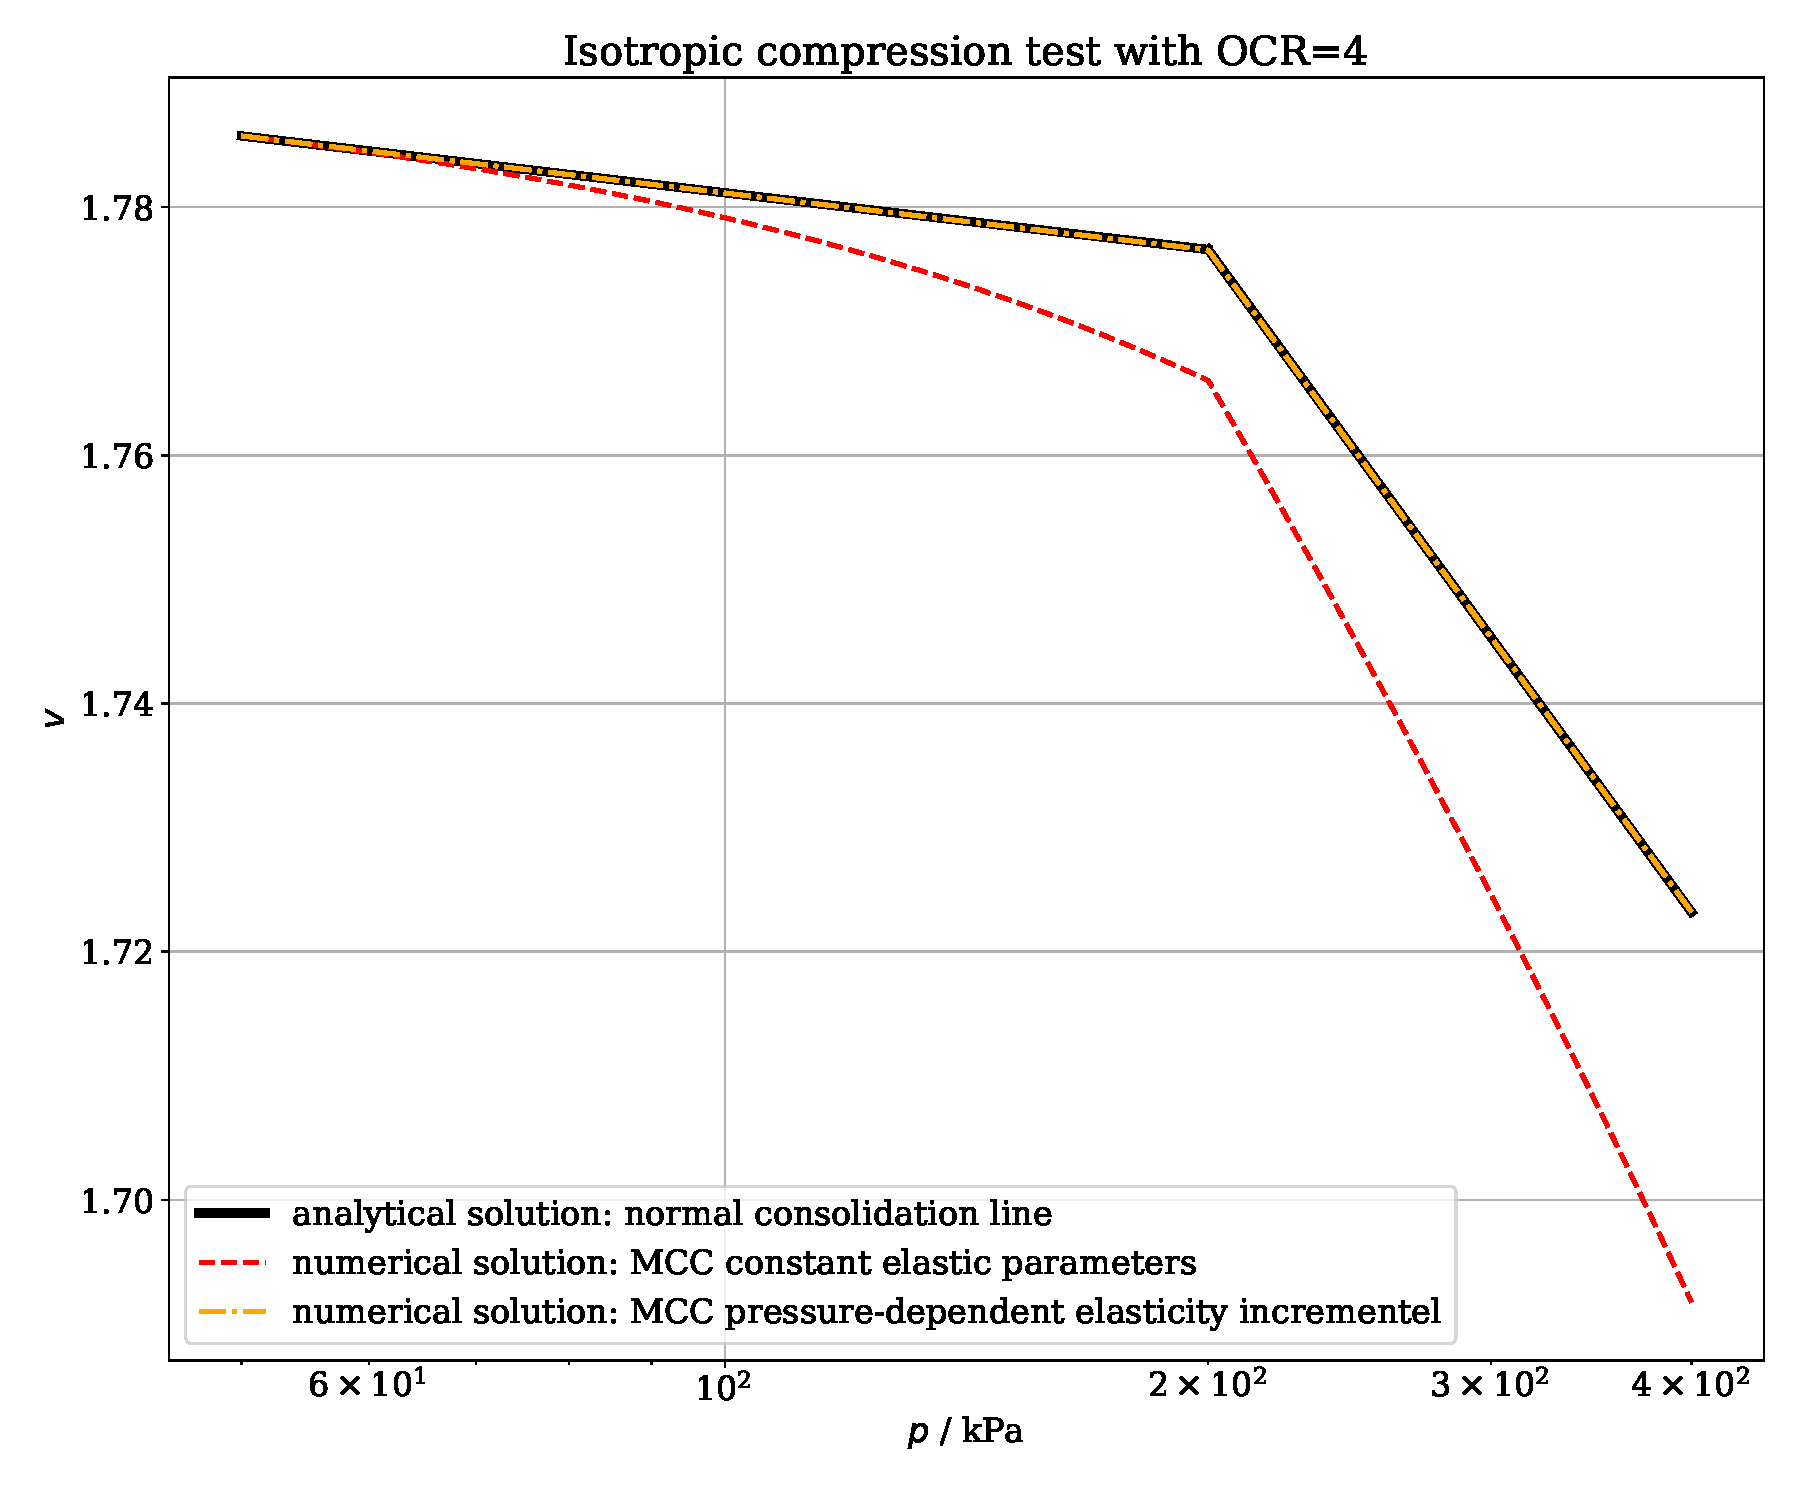
\includegraphics[width=0.8\textwidth]{img/SemiExplicitModifiedCamClay_OpenGeoSys2023/Comparison_NCL_MCC_new_OCR=4.pdf}
  \caption{Normal consolidation line: analytical and numerical solution for the original MCC model (pressure-dependent elasticity) versus numerical solution with the basic version (constant elastic parameters). Note the logarithmic p-axis.}\label{fig:Comparison_NCL_MCC_OCR}
\end{figure}
\par
\autoref{fig:Comparison_NCL_MCC_OCR} shows the perfect fit of analytical and numerical solution for the original MCC model \ref{subsec:ImplementationOriginal} with pressure-dependent elastic parameters. However, the version \ref{subsec:ImplementationConstE} with constant elastic parameters (cf. \autoref{subsec:linear_elastic}) significantly deviates. Hence, the basic version should not be used for this kind of test (if the typical Cam clay behavior is expected). Instead, the basic version can be used very well if stress paths with high deviatoric proportion are present (cf. triaxial test in \autoref{subsec:triaxialCompression}).

\subsection{Consolidated plane strain simple shear test using \textsl{mtest}}\label{subsec:mtestResults}

In order to test the consolidation behaviour, plane strain simple shear tests were conducted with the same initial state but three different loading trajectories. To be precise, first the hydrostatic pressure $p$ was increased until $0.25\,p_{\c0}, 0.5\,p_{\c0}$ or $0.75\,p_{\c0}$. This results in the overconsolidation ratios (OCR $=p_{\c0}/p$) of $4, 2, 4/3$. From this hydrostatic stress state, shear is applied up to the strain $\varepsilon_{xy}=0.01$.

%OCR=1 means normally consolidated, OCR>1 describes an over-consolidated state
%OCR=maximum pressure (=pre-consolidation pressure) / current pressure

\begin{table}[h!]
  \centering
  \caption{Material parameters for the modified Cam clay model implementation \ref{subsec:ImplementationConstE}}
  \label{tab:matParaCamClay}
  \begin{tabular}{c c c c c c c c c c}
  \firsthline
    {$E$} / Pa & {$\nu$} & {$M$} & {$\lambda$} & {$\kappa$} & {$v_0$} & {$p_{\c0}$} / Pa & {$p_\text{amb}$} / Pa\\
    \hline
    $150\cdot10^{9}$ & $0.3$ & $1.5$ & $7.7\cdot 10^{\minus3}$ & $6.6\cdot 10^{\minus4}$ & $1.788$ & $30\cdot10^{6}$ & $0\cdot10^{3}$ \\
    \lasthline
  \end{tabular}
\end{table}
Implementation \ref{subsec:ImplementationConstE} is used, material parameters and initial values are given in \autoref{tab:matParaCamClay}. Note that only the difference $\lambda - \kappa$ plays a role in the implementation with \emph{constant} elastic parameters. Considering the OCR, there are three different cases (cf. \autoref{fig:mtestShear3cases}):
%\vspace{-2mm}
\begin{figure}[h!]
  \hspace{-10mm}
  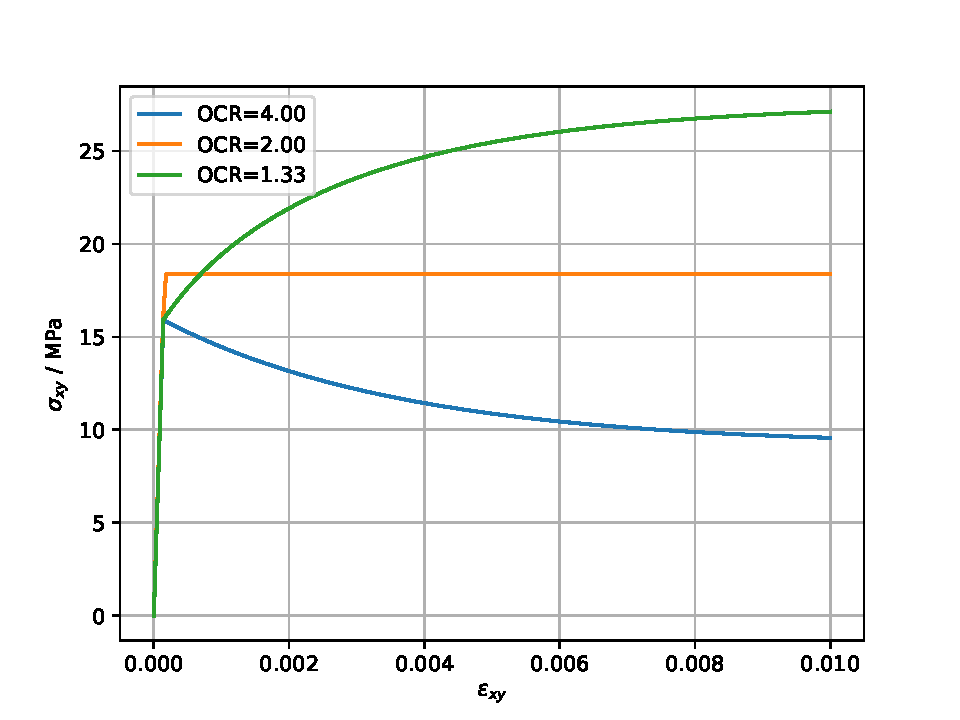
\includegraphics[width=0.60\textwidth]{img/SemiExplicitModifiedCamClay_OpenGeoSys2023/ModCamClay_ParamStudy_ShearCurves_pStudy}
  \hspace{-10mm}
  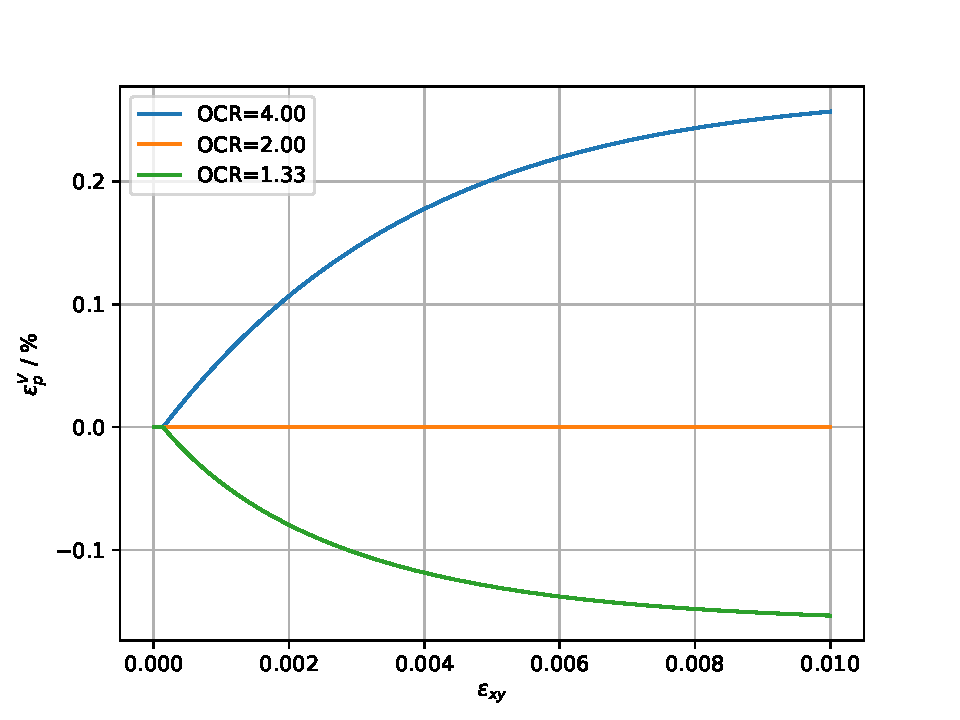
\includegraphics[width=0.60\textwidth]{img/SemiExplicitModifiedCamClay_OpenGeoSys2023/ModCamClay_ParamStudy_eplVCurves_pStudy}
  \caption{Consolidated shear test for three typical OCR values: $\varepsilon_\p^\text{V}>0$ causes softening, whereas $\varepsilon_\p^\text{V}<0$ (compaction) results in hardening.}\label{fig:mtestShear3cases}
\end{figure}
For $\text{OCR}>2$ the shearing is accompanied by a plastic expansion (dilatancy) with $\varepsilon_\p^\text{V}>0$, which is related to softening until the critical state is reached.
\par
For $\text{OCR}=2$ shearing until yield leads directly to the critical state. Considering the state of the soil (porosity, stress, volume) this is a natural asymptotic state. Further shearing does not alter that state anymore. Hence, there is ideal plastic behaviour.
\par
For $\text{OCR}<2$ the shearing is accompanied by a plastic compaction (contractant flow, consolidation) with $\varepsilon_\p^\text{V}<0$, which is related to hardening until the critical state is reached.
\par
\noindent
The stress trajectories, and the final yield surfaces are illustrated in the $p,q$-space together with the initial yield surface and the critical state line (CSL).
\begin{figure}[h!]\centering
  \vspace{-26mm}
  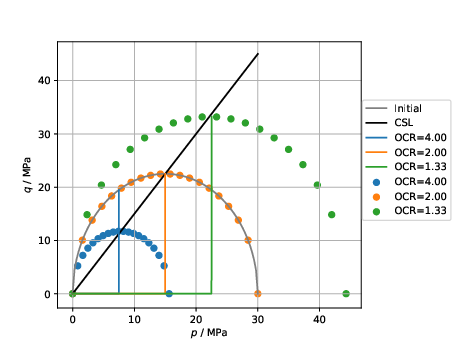
\includegraphics[width=0.61\textwidth]{img/SemiExplicitModifiedCamClay_OpenGeoSys2023/ModCamClay_ParamStudy_YieldSurface_pStudy}
  \caption{Consolidated shear test for 3 typical OCR values: depicted are the different stress trajectories, the critical state line (CSL) and the final yield surfaces.}\label{fig:mtestShear3casesYield}
\end{figure}
\par
\noindent
Now, the same consolidated shear loading is applied, but with two different initial states: a high initial pre-consolidation pressure $p_{\c0}$ resembles a heavily pre-consolidated, compacted (dense) soil material, whereas a low value of $p_{\c0}$ resembles a loosened initial state. 
\begin{figure}[h!]
  \vspace{-6mm}
  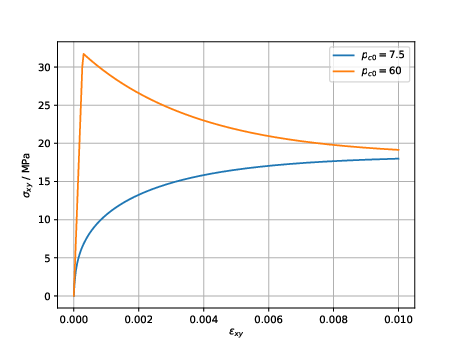
\includegraphics[width=0.52\textwidth]{img/SemiExplicitModifiedCamClay_OpenGeoSys2023/ModCamClay_ParamStudy_ShearCurves_pcStudy}
  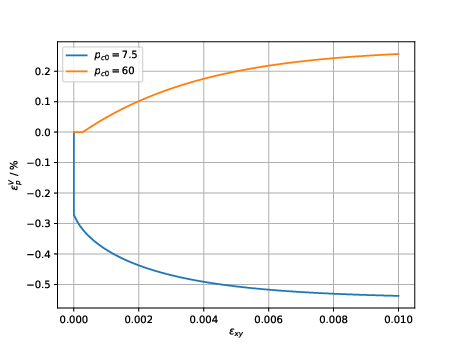
\includegraphics[width=0.52\textwidth]{img/SemiExplicitModifiedCamClay_OpenGeoSys2023/ModCamClay_ParamStudy_eplVCurves_pcStudy}
  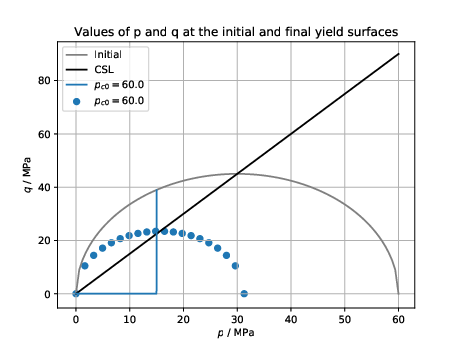
\includegraphics[width=0.52\textwidth]{img/SemiExplicitModifiedCamClay_OpenGeoSys2023/ModCamClay_ParamStudy_YieldSurface_pcHigh}
  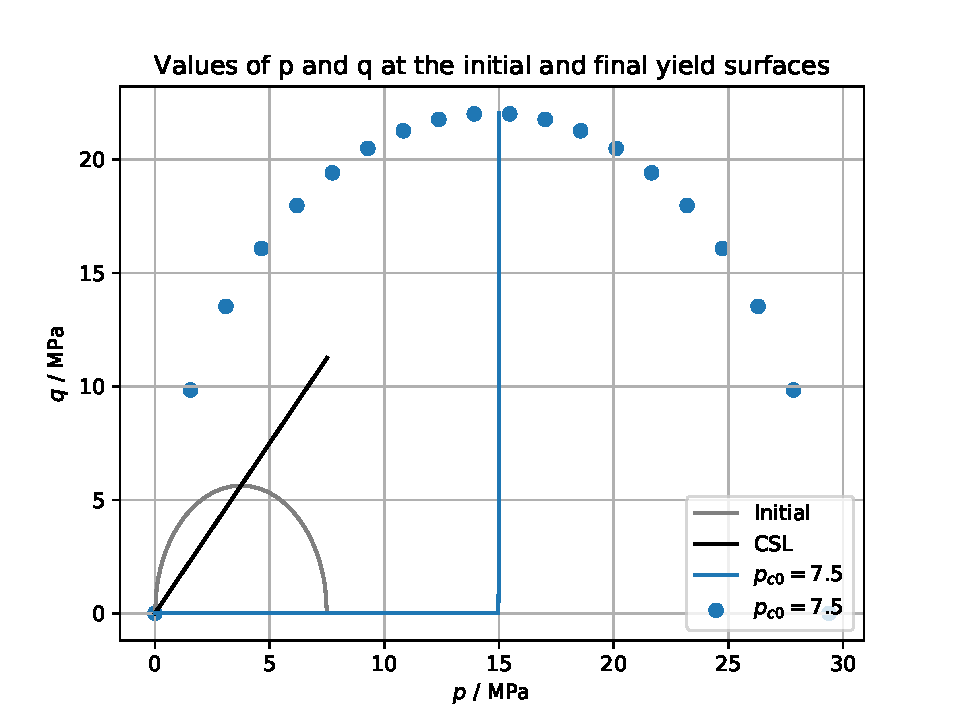
\includegraphics[width=0.52\textwidth]{img/SemiExplicitModifiedCamClay_OpenGeoSys2023/ModCamClay_ParamStudy_YieldSurface_pcLow}
  \caption{Consolidated shear test for two different initial pre-consolidation pressures: the CSL and the final state including the final yield surface are equal.}\label{fig:mtestShear2cases}
\end{figure}
\par
\noindent
As can be seen in \autoref{fig:mtestShear2cases} the materials strive to the same (asymptotic) critical state, since the CSL is identical. However, this is either accomplished by hardening (contraction) or softening (dilatancy).
\iffalse
\begin{figure}[h!]
  \hspace{-10mm}
  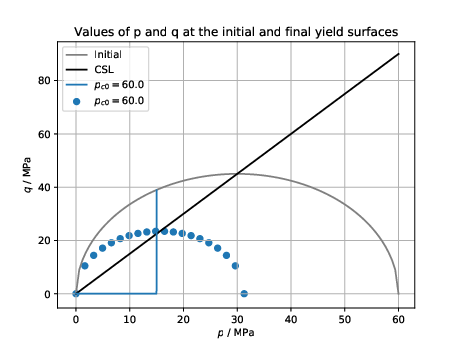
\includegraphics[width=0.58\textwidth]{img/SemiExplicitModifiedCamClay_OpenGeoSys2023/ModCamClay_ParamStudy_YieldSurface_pcHigh}
  \hspace{-10mm}
  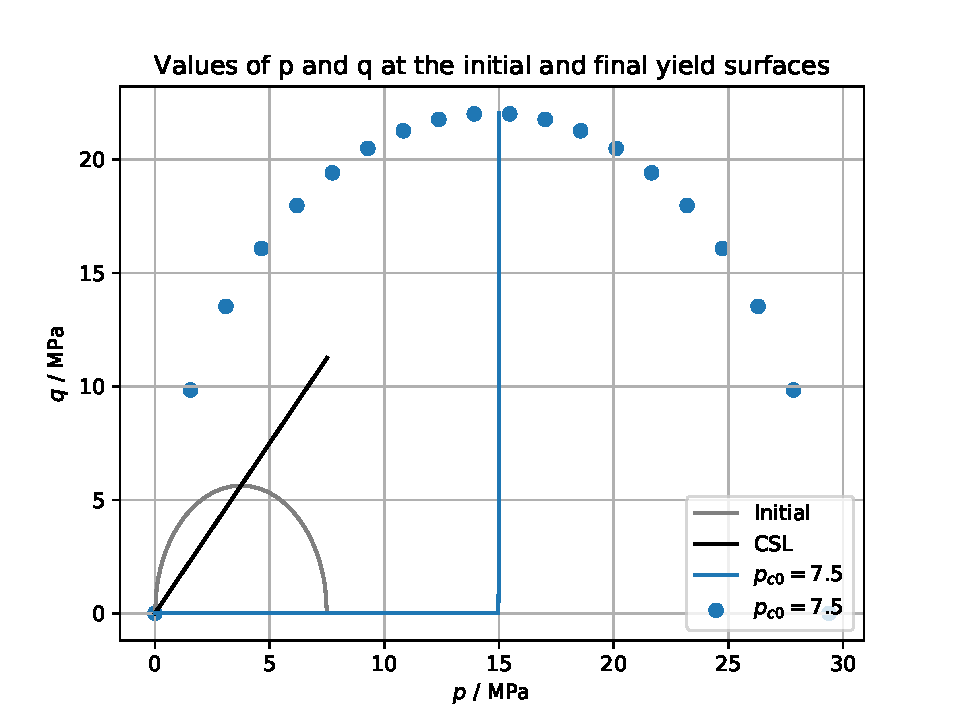
\includegraphics[width=0.58\textwidth]{img/SemiExplicitModifiedCamClay_OpenGeoSys2023/ModCamClay_ParamStudy_YieldSurface_pcLow}
\caption{Consolidated shear test for two different initial pre-consolidation pressures: the CSL and the final state including the final yield surface are equal.}\label{fig:mtestShear2casesYield}
\end{figure}
\fi

\subsection{Plane strain simple shear test with one FE using \textsl{OpenGeoSys}}

As a next step the shear test from the previous section was repeated using \textsl{OpenGeoSys} and model \ref{subsec:ImplementationConstE}, but without consolidation phase. A unit square domain was meshed with only one finite element. At the boundaries (top, bottom, left, right) Dirichlet boundary conditions~(BCs) were prescribed. The top boundary was loaded by a linear displacement ramp from time $0$ to $1\,$s. The material parameters were taken from \autoref{tab:matParaCamClay} with only one difference: As the test has no pre-consolidation phase, it starts from zero stress and due to the reasons explained in \autoref{subsec:stabilization} some small ambient pressure $p_\text{amb}=10^{3}$\,Pa was added.\footnote{If the test is stress-controlled and the material is initially on the critical state with zero stress, this causes an infinite strain increment and no convergence can be expected.}

\begin{table}[h!]
  \begin{tabular}{l|c|c|l|c|r}
     Test                    & BC left   & BC right      & BC top               & BC bottom   & behaviour\\
     \hline
     Shear $xy$         & free      & free          & $u_x=-v t, u_y=0$  & $u_x=u_y=0$ & convergence\\
     Shear $xy$         & free      & free          & $u_x=-v t$         & $u_x=u_y=0$ & no convergence\\
%     Shear $xy$ + compr. $y$ & free      & free          & $u_x=u_y=-0.05t$     & $u_x=u_y=0$ & convergence\\
     \hline 
  \end{tabular}
  \caption{Convergence behaviour for different BCs, $v=0.05$ m/s, $t$ is the time.}\label{table:shear1FE}
\end{table}

\begin{figure}[h]
  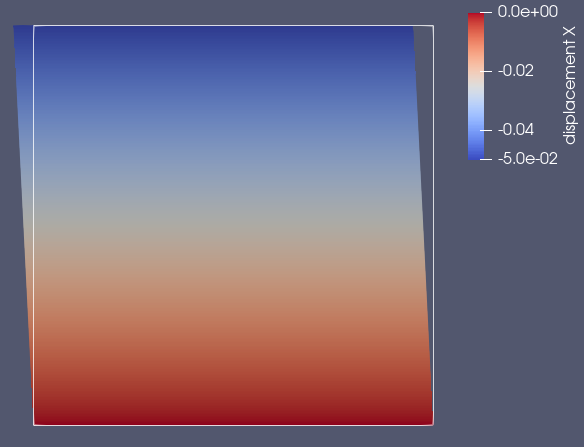
\includegraphics[width=0.5\textwidth]{img/SemiExplicitModifiedCamClay_OpenGeoSys2023/SimpleShearCamClay_uyTop=0.png}
  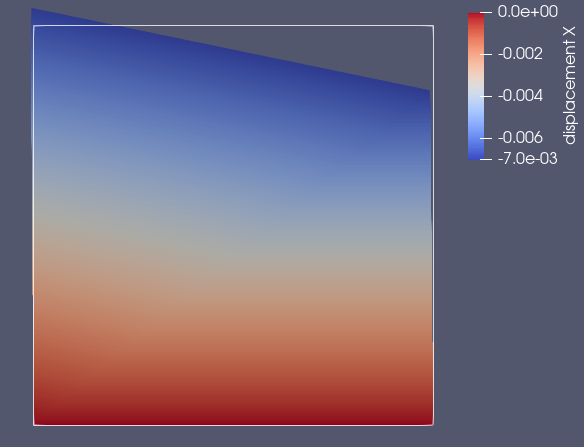
\includegraphics[width=0.5\textwidth]{img/SemiExplicitModifiedCamClay_OpenGeoSys2023/SimpleShearCamClay_freeTop.png}
  \caption{Test results for different BCs according to \autoref{table:shear1FE}: the top boundary is either confined (\textsl{left}) or free (\textsl{right}). }\label{fig:shear1FE}
\end{figure}

In order to have true simple shear, the top BC $u_y=0$ has to be applied. Else there is a tilting effect, and the deformation consists of shear and bending. As this is related to some parts with dominant tension stresses, convergence cannot be achieved with the Cam clay model (cf. next section). Note also that for pure shear $\varepsilon^\text{V}=0$ and the volume and porosity thus remain constant. %(even for $\varepsilon^\text{V}\neq 0$)


\subsection{Plane strain simple biaxial test with one FE using \textsl{OpenGeoSys}}

It must be noted that the Cam clay model is primarily intended to capture the shear behaviour of soil materials \emph{without} tensile strength. Hence, the uniaxial stress states with free boundaries cannot be sustained just as these states cannot be reached in reality. As an example, uniaxial tension causes pronounced lateral stretching due to plastic volume increase (dilatancy). The application of some minimal pre-consolidation pressure can help to stabilize the simulation, but convergence cannot be expected in general.
\par
Still, the biaxial tension/compression behaviour can be simulated to a certain degree. Material parameters and setup are the same as in the previous section. \autoref{table:biaxial1FE} shows under which conditions convergence can be expected. In the converged cases a homogeneous solution was obtained as expected.

\begin{table}[h!]
  \begin{tabular}{l|l|c|c|c|c|c}
     No & Test                    & BC left   & BC right      & BC top               & BC bottom   & convergence\\
     \hline
     1 & Uniax. compr. $y$       & $u_x=0$   & free       & $u_y=-v t$         & $u_y=0$     & no\\
     2 & Uniax. tension $y$      & $u_x=0$   & free       & $u_y=+v t$         & $u_y=0$     & no\\
     3 & Biaxial compr. $x,y$    & $u_x=0$   & $u_x=-v t$ & $u_y=-v t$         & $u_y=0$     & yes\\
     4 & Biaxial tension $x,y$   & $u_x=0$   & $u_x=+v t$ & $u_y=+v t$         & $u_y=0$     & (yes)\\
     5 & Biaxial mixed $x,y$     & $u_x=0$   & $u_x=+v t$ & $u_y=-v t$         & $u_y=0$     & yes\\
     6 & Biaxial mixed $x,y$     & $u_x=0$   & $u_x=-v t$ & $u_y=+v t$         & $u_y=0$     & yes\\
     \hline 
  \end{tabular}
  \caption{Convergence behaviour for different biaxial loadings and BCs, $v=0.05$ m/s.}\label{table:biaxial1FE}
\end{table}

It is interesting to note that the biaxial tension test can be simulated with the Cam clay model. In order to achieve convergence the drop of the pre-consolidation pressure has to be limited. For this, either the value of the parameter difference $\lambda - \kappa$ is increased or some minimal value $p^\text{min}_\c$ has to be ensured according to Eq.~\eqref{eq:pcMin}.

\begin{figure}[h]
  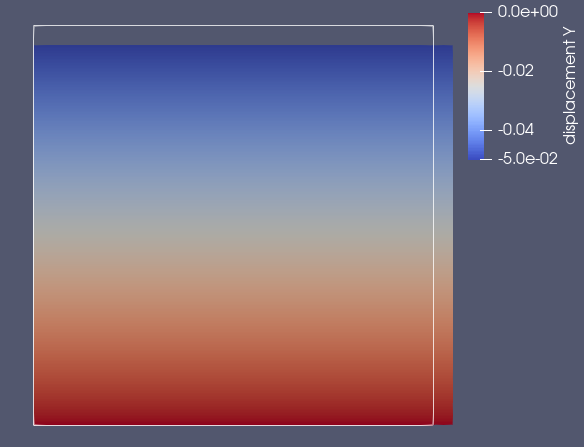
\includegraphics[width=0.5\textwidth]{img/SemiExplicitModifiedCamClay_OpenGeoSys2023/BiaxtestCamClay_TopComprRightTension.png}
  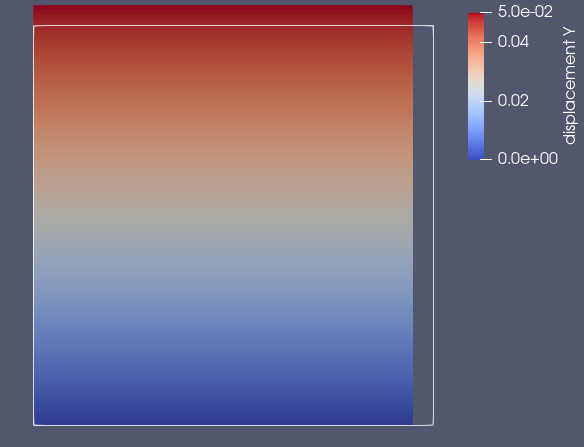
\includegraphics[width=0.5\textwidth]{img/SemiExplicitModifiedCamClay_OpenGeoSys2023/BiaxtestCamClay_TopTensionRightCompr.png}
  \caption{Biaxial test results for different BCs: shown are the mixed cases from \autoref{table:biaxial1FE}, \textsl{left}) test number 5 and \textsl{right}) test number 6.}\label{fig:biaxMixedCases}
\end{figure}


\subsection{Axially-symmetric triaxial compression test}\label{subsec:triaxialCompression}

As a benchmark to existing results an axially-symmetric triaxial compression test was performed. For this, a cylindrical domain of height $100$\,m and radius $25$\,m is meshed with $100\times 25$ finite elements. At the left and bottom boundaries symmetry BCs of Dirichlet type are prescribed. The top and right boundaries are loaded by prescribing an axial and a confining pressure $p_{\text{con}}$, respectively. The loading starts from a hydrostatic stress state with $p_0=p_{\text{con}}=p_{\c0}$ (normally consolidated, i.\,e. OCR=$1$). Then the axial pressure is increased while the confining pressure $p_{\text{con}}$ is held constant. As the simulation time is irrelevant, it is again set to $1\,$s. The material parameters are taken from \autoref{tab:matParaCamClay0} and the same settings are applied in order to compare the \emph{original} Modified Cam Clay model \ref{subsec:ImplementationOriginal} and the implementation with constant elastic parameters \ref{subsec:ImplementationConstE}. According to Eq. \eqref{eq:relationE-kappa} the (initial) Young's modulus is thus
$$
E_0 = 3(1-2\nu) \frac{v_0}{\kappa} p_{c0}= 64.9345~\text{MPa} \ ,
$$
which is a reasonable value. The displacement field is illustrated in \autoref{fig:triaxDisplacement}.
\begin{figure}[h!]\centering
  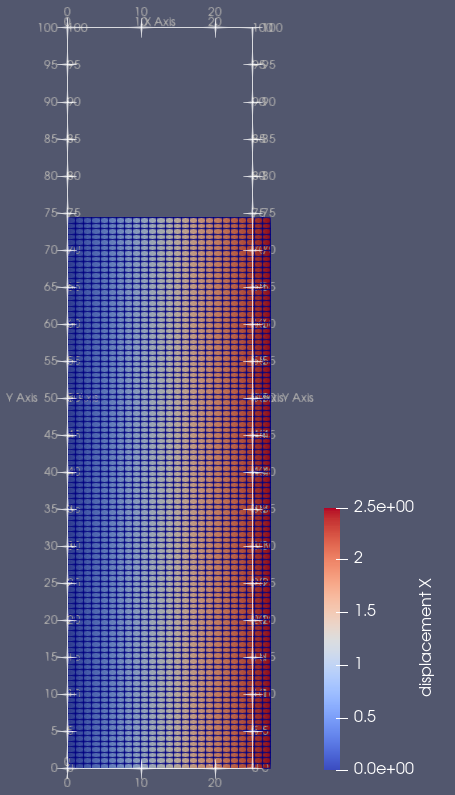
\includegraphics[width=0.45\textwidth]{img/SemiExplicitModifiedCamClay_OpenGeoSys2023/TriaxCamClay_StressControl_ux.png}\vspace{10mm}
  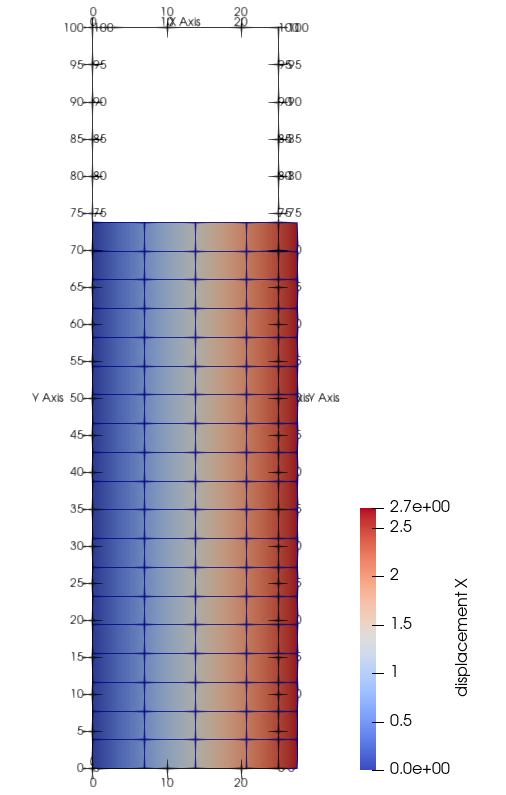
\includegraphics[width=0.45\textwidth]{img/SemiExplicitModifiedCamClay_OpenGeoSys2023/TriaxCamClay_StressControl_ux_Original.png}
  \vspace{-3mm}
  \caption{Triaxial benchmark results: shown are the displacement coefficients in the radial (here $x$) direction, \textsl{left} implementation \ref{subsec:ImplementationConstE} and \textsl{right} \ref{subsec:ImplementationOriginal}.
  }\label{fig:triaxDisplacement}
\end{figure}
\par
\noindent
Since the stress and strain fields are homogeneous, it is sufficient to further analyze the solution at some arbitrary integration point.
The material and loading parameters were chosen such that the stress trajectory approaches the CSL from the right side but does not meet it (cf. \autoref{fig:triaxStressTrajectory}). Otherwise there will be zero resistance to plastic flow causing an infinite strain increment in the stress-controlled test and no convergence can be expected. The tendency can already be seen in \autoref{fig:triaxStressStrainConstE}/\ref{fig:triaxStressStrainOriginal} (right) with the steep increase of the equivalent plastic strain. The curve of the pre-consolidation pressure (cf. \autoref{fig:triaxStressStrainConstE}/\ref{fig:triaxStressStrainOriginal} left) shows monotonic hardening related to plastic compaction (cf. plastic volumetric strain in  \autoref{fig:triaxStressStrainConstE}/\ref{fig:triaxStressStrainOriginal} right).
\begin{figure}[h!]
  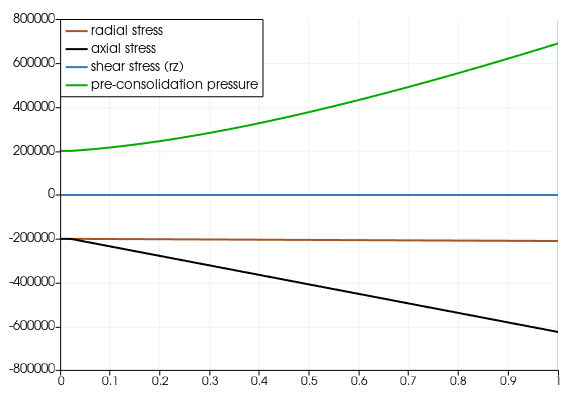
\includegraphics[width=0.52\textwidth]{img/SemiExplicitModifiedCamClay_OpenGeoSys2023/TriaxCamClay_StressControl_StressCurves.png}
  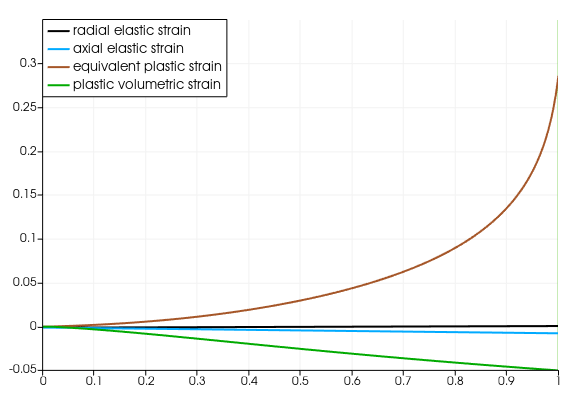
\includegraphics[width=0.52\textwidth]{img/SemiExplicitModifiedCamClay_OpenGeoSys2023/TriaxCamClay_StressControl_StrainCurves.png}
  \caption{Triaxial benchmark results using implementation \ref{subsec:ImplementationConstE}: shown is the evolution of stress (\textsl{left}, unit Pa) and strain measures (\textsl{right}) at some integration point.}\label{fig:triaxStressStrainConstE}
\end{figure}
\begin{figure}[h!]
  \vspace{-6mm}
  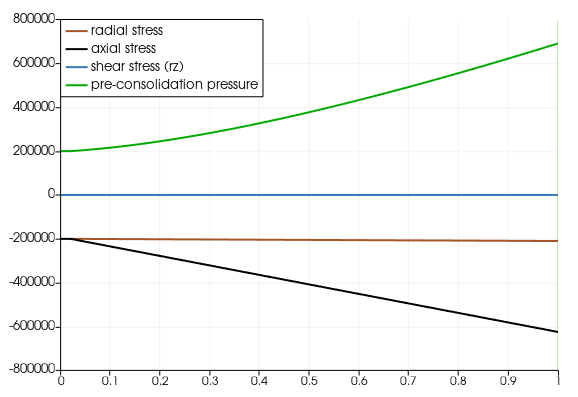
\includegraphics[width=0.52\textwidth]{img/SemiExplicitModifiedCamClay_OpenGeoSys2023/TriaxCamClay_StressControl_StressCurves_Original.png}
  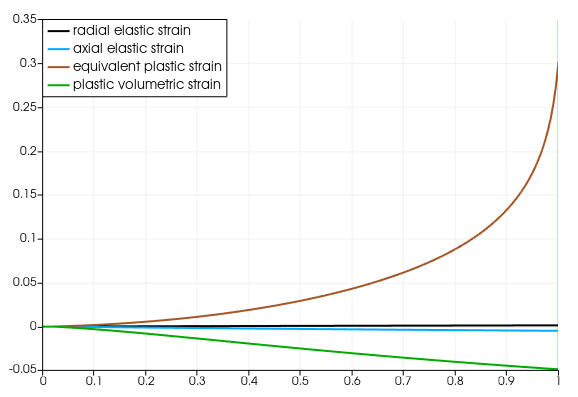
\includegraphics[width=0.52\textwidth]{img/SemiExplicitModifiedCamClay_OpenGeoSys2023/TriaxCamClay_StressControl_StrainCurves_Original.png}
  \caption{Triaxial benchmark results using implementation \ref{subsec:ImplementationOriginal}: shown is the evolution of stress (\textsl{left}, unit Pa) and strain measures (\textsl{right}) at some integration point.}\label{fig:triaxStressStrainOriginal}
\end{figure}
\par
\noindent
Comparing \autoref{fig:triaxStressStrainConstE} with \autoref{fig:triaxStressStrainOriginal} it can be seen that the solutions are not identical but close to each other, showing the applicability of the implementation \ref{subsec:ImplementationConstE} for this kind of test. The reason is the pronounced deviatoric stress component -- in contrast to the pure isotropic compression test (cf. \autoref{subsec:consolidationLine}).
\begin{figure}[h!]\centering
  \vspace{-12mm}
  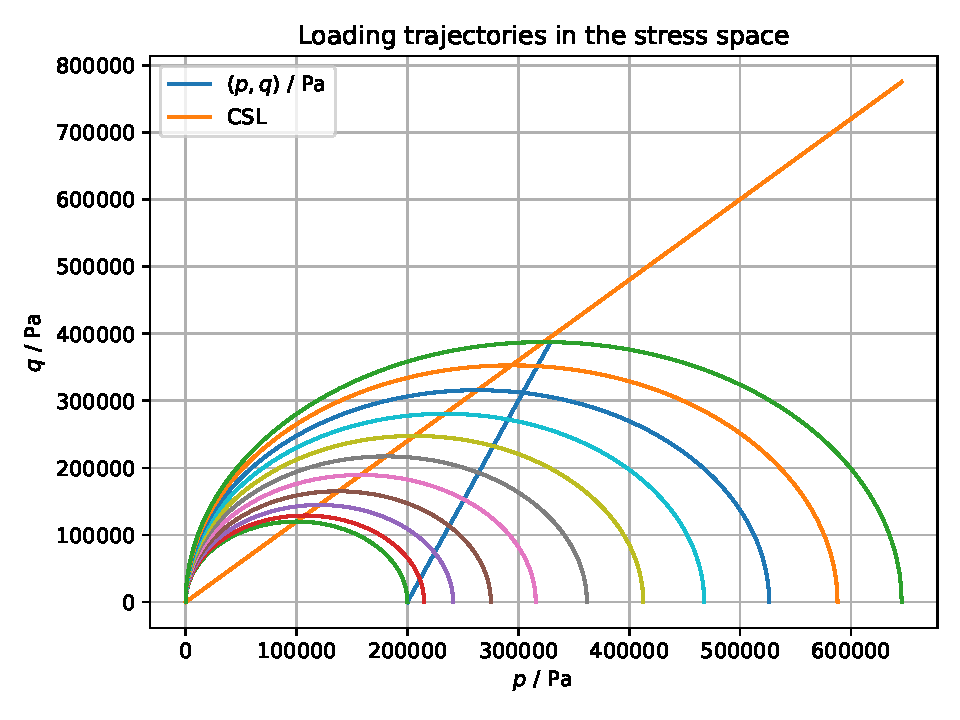
\includegraphics[width=0.7\textwidth]{img/SemiExplicitModifiedCamClay_OpenGeoSys2023/ModCamClay_TriaxStudy_YieldSurface_41.pdf}
  \caption{Triaxial benchmark results using implementation \ref{subsec:ImplementationConstE}: depicted is the stress trajectory and the evolving yield surface as well as the CSL.}\label{fig:triaxStressTrajectory}
\end{figure}
\par
%\noindent
In order to check the accuracy of the numerical results, they were compared to an analytical solution \cite{Peric2006} for proportional loading (cf. Appendix \ref{subsec:AppSolutionPeric}). For this, the straight stress path starting from $(p, q) = (p_{\c0}, 0)$ until the final state $(p, q)=(387387, 330129)\ $Pa is considered (cf. \autoref{fig:triaxStressTrajectory}). Plotting the von-Mises stress over the corresponding equivalent strain defined by $\varepsilon_{\text{q}}^2= {\tfrac{2}{3}\ \tensor\varepsilon^\D\ppkt\tensor\varepsilon^\D}$ shows the agreement between numerical and analytical solution.
\par
\begin{figure}[h!]
  %\vspace{-6mm}
  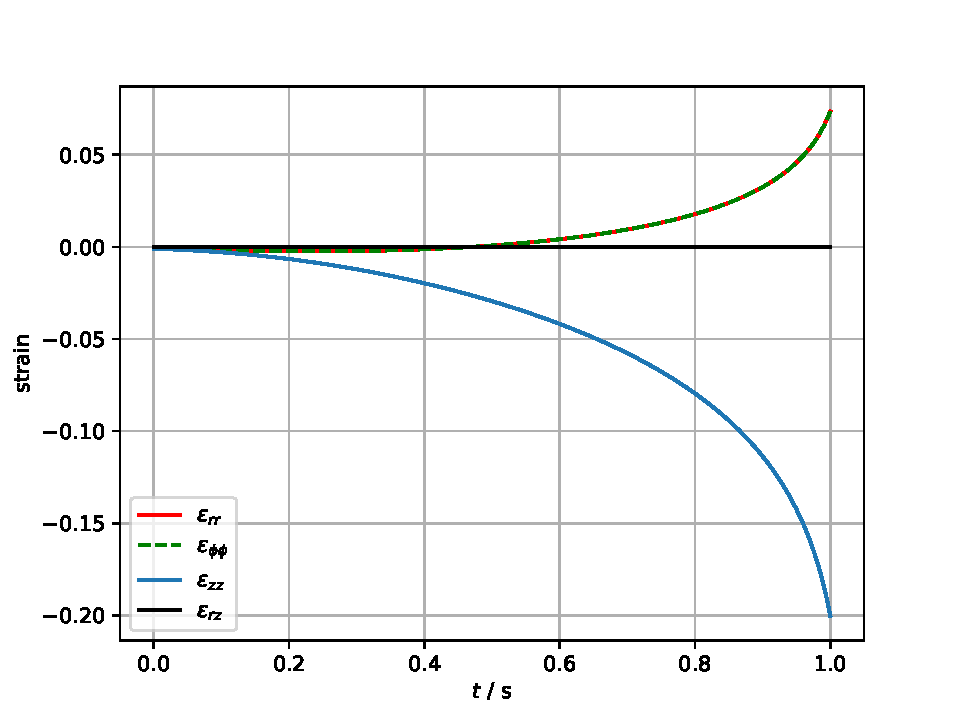
\includegraphics[width=0.52\textwidth]{img/SemiExplicitModifiedCamClay_OpenGeoSys2023/ModCamClay_TriaxStudy_Strains_41.pdf}
  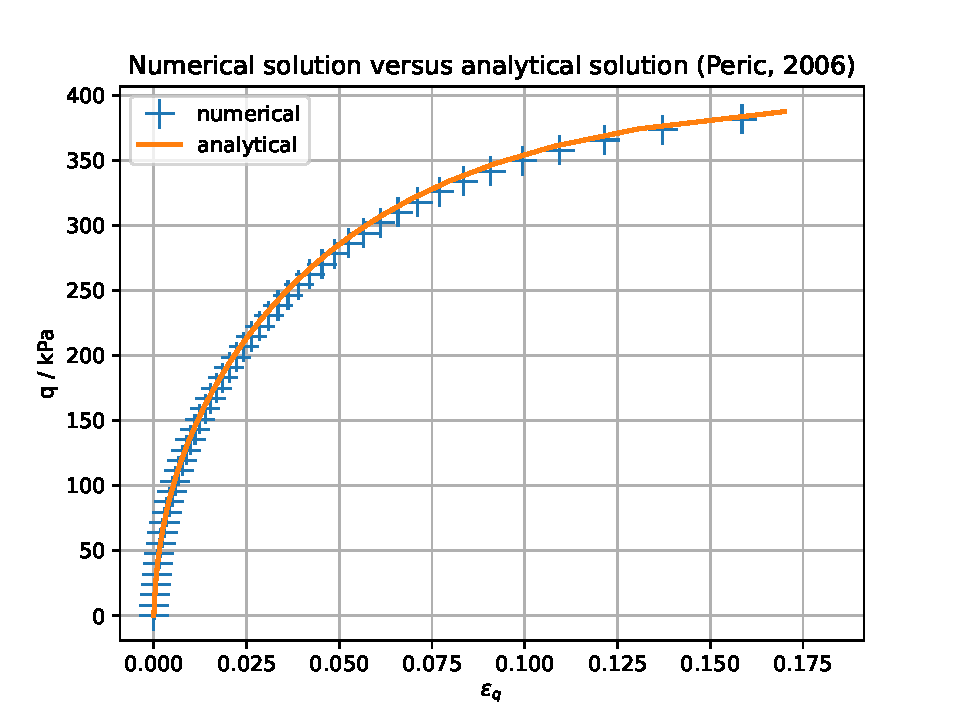
\includegraphics[width=0.52\textwidth]{img/SemiExplicitModifiedCamClay_OpenGeoSys2023/ModCamClay_TriaxStudy_NumVsAnal_41.pdf}
  \caption{Triaxial benchmark results using implementation \ref{subsec:ImplementationConstE}: depicted are the strains (\textsl{left}) and a comparison between analytical and numerical solution (\textsl{right}).}\label{fig:triaxStressStrains}
\end{figure}
\begin{figure}[h!]
  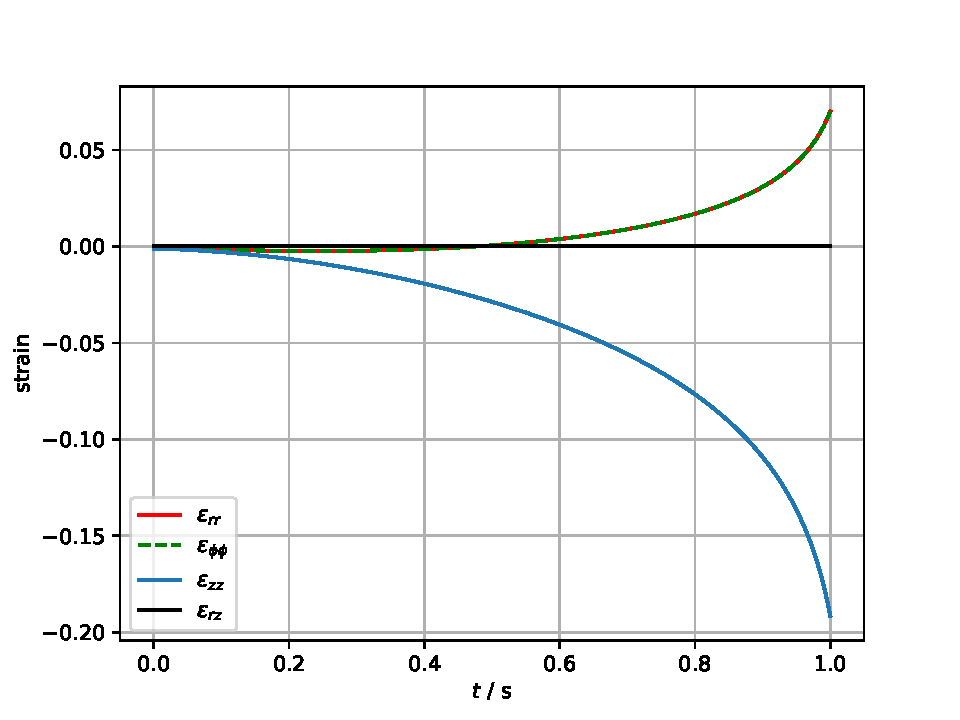
\includegraphics[width=0.52\textwidth]{img/SemiExplicitModifiedCamClay_OpenGeoSys2023/ModCamClay_TriaxStudy_Strains_42.pdf}
  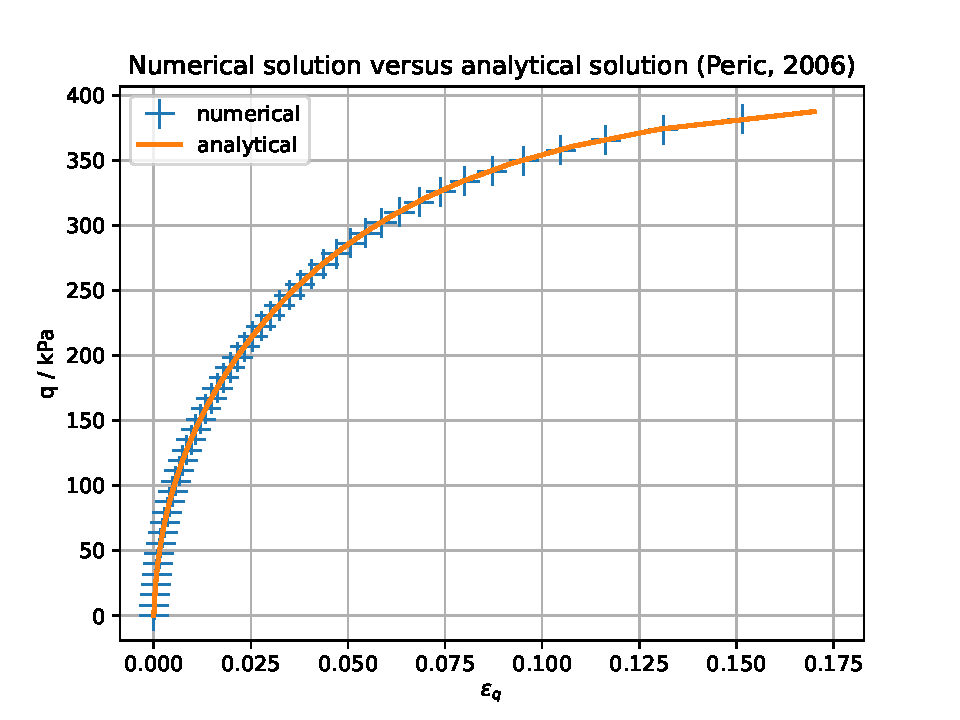
\includegraphics[width=0.52\textwidth]{img/SemiExplicitModifiedCamClay_OpenGeoSys2023/ModCamClay_TriaxStudy_NumVsAnal_42.pdf}
  \caption{Triaxial benchmark results using implementation \ref{subsec:ImplementationOriginal}: depicted are the strains (\textsl{left}) and a comparison between analytical and numerical solution (\textsl{right}).}\label{fig:triaxStressStrainsOriginal}
\end{figure}
\noindent
Using the implementation \ref{subsec:ImplementationConstE}, minor deviations arise from the assumption of a constant bulk modulus according to Eq. \eqref{eq:constK} (cf. \autoref{fig:triaxStressStrains} right). The original implementation \ref{subsec:ImplementationOriginal} using the pressure-dependent bulk modulus according to Eq. \eqref{eq:elasticParameters}, on the other hand, shows perfect agreement with the analytical solution (cf. \autoref{fig:triaxStressStrainsOriginal} right).
\par
\noindent
Considering the radial and circumferential strains another peculiarity is found (cf. \autoref{fig:triaxStressStrains}): The initial plastic compaction causes lateral (i.\,e. radial and circumferential) contraction. However, with increasing axial compression this necessarily turns into expansion. Note also that for this \emph{numerical} test the magnitude of the strains is beyond the scope of the linear strain measure.
%remark on large strains: linear strain measure, physically not meaningful, but numerical test

As an alternative, the test could also be conducted displacement-controlled. However, in doing so it was found that the homogeneous solution becomes unstable and strain localization occurs at the top of the domain. Apparently, at some integration points softening sets in even though the homogeneous solution only shows monotonic hardening. Varying the mesh size and topology, convergence could be achieved in some cases, indicating a strong mesh dependency.

\section{Concluding remarks}

The presented Cam clay material model has a simple structure, but can capture several characteristic phenomena of soil materials very well. However, it must be considered with caution when applied to realistic finite element simulations. The major limitations have two origins: first, the missing cohesion and second, the dilatant/softening part of the captured material behaviour. The provided numerical refinements can stabilize this only to a limited degree. It seems that the softening can cause a pronounced strain localization, which requires special strategies for regularization of the underlying ill-posed mathematical problem \cite[cf. e.\,g.][]{Manica2018}. In order to include finite cohesion different modifications of the Cam clay model have been proposed \cite[cf. e.\,g.][]{Gaume2018}. Finally, mechanical loading in the vicinity of the critical state can easily cause large deformations, a finite strain formulation should be considered in the future \cite[cf. e.\,g.][]{Borja1998,Callari1998}.


\appendix

\section{Appendix}

\subsection{Numerical convergence behavior of the basic Modified Cam clay implementation}
\label{subsec:AppConvergence}

In order to check the convergence rate of the Cam clay implementation \ref{subsec:ImplementationConstE} the consolidated shear test from Section~\ref{subsec:mtestResults} was considered again. The parameters were taken from \autoref{tab:matParaCamClay}. The hydrostatic pressure $p$ was increased until $0.66\,p_{\c0}$ resulting in an OCR of $1.5$. From this hydrostatic stress state, shear is applied up to the strain $\varepsilon_{xy}=5\cdot10^{-4}$ within $20$ time steps.

\begin{figure}[h!]%\centering
  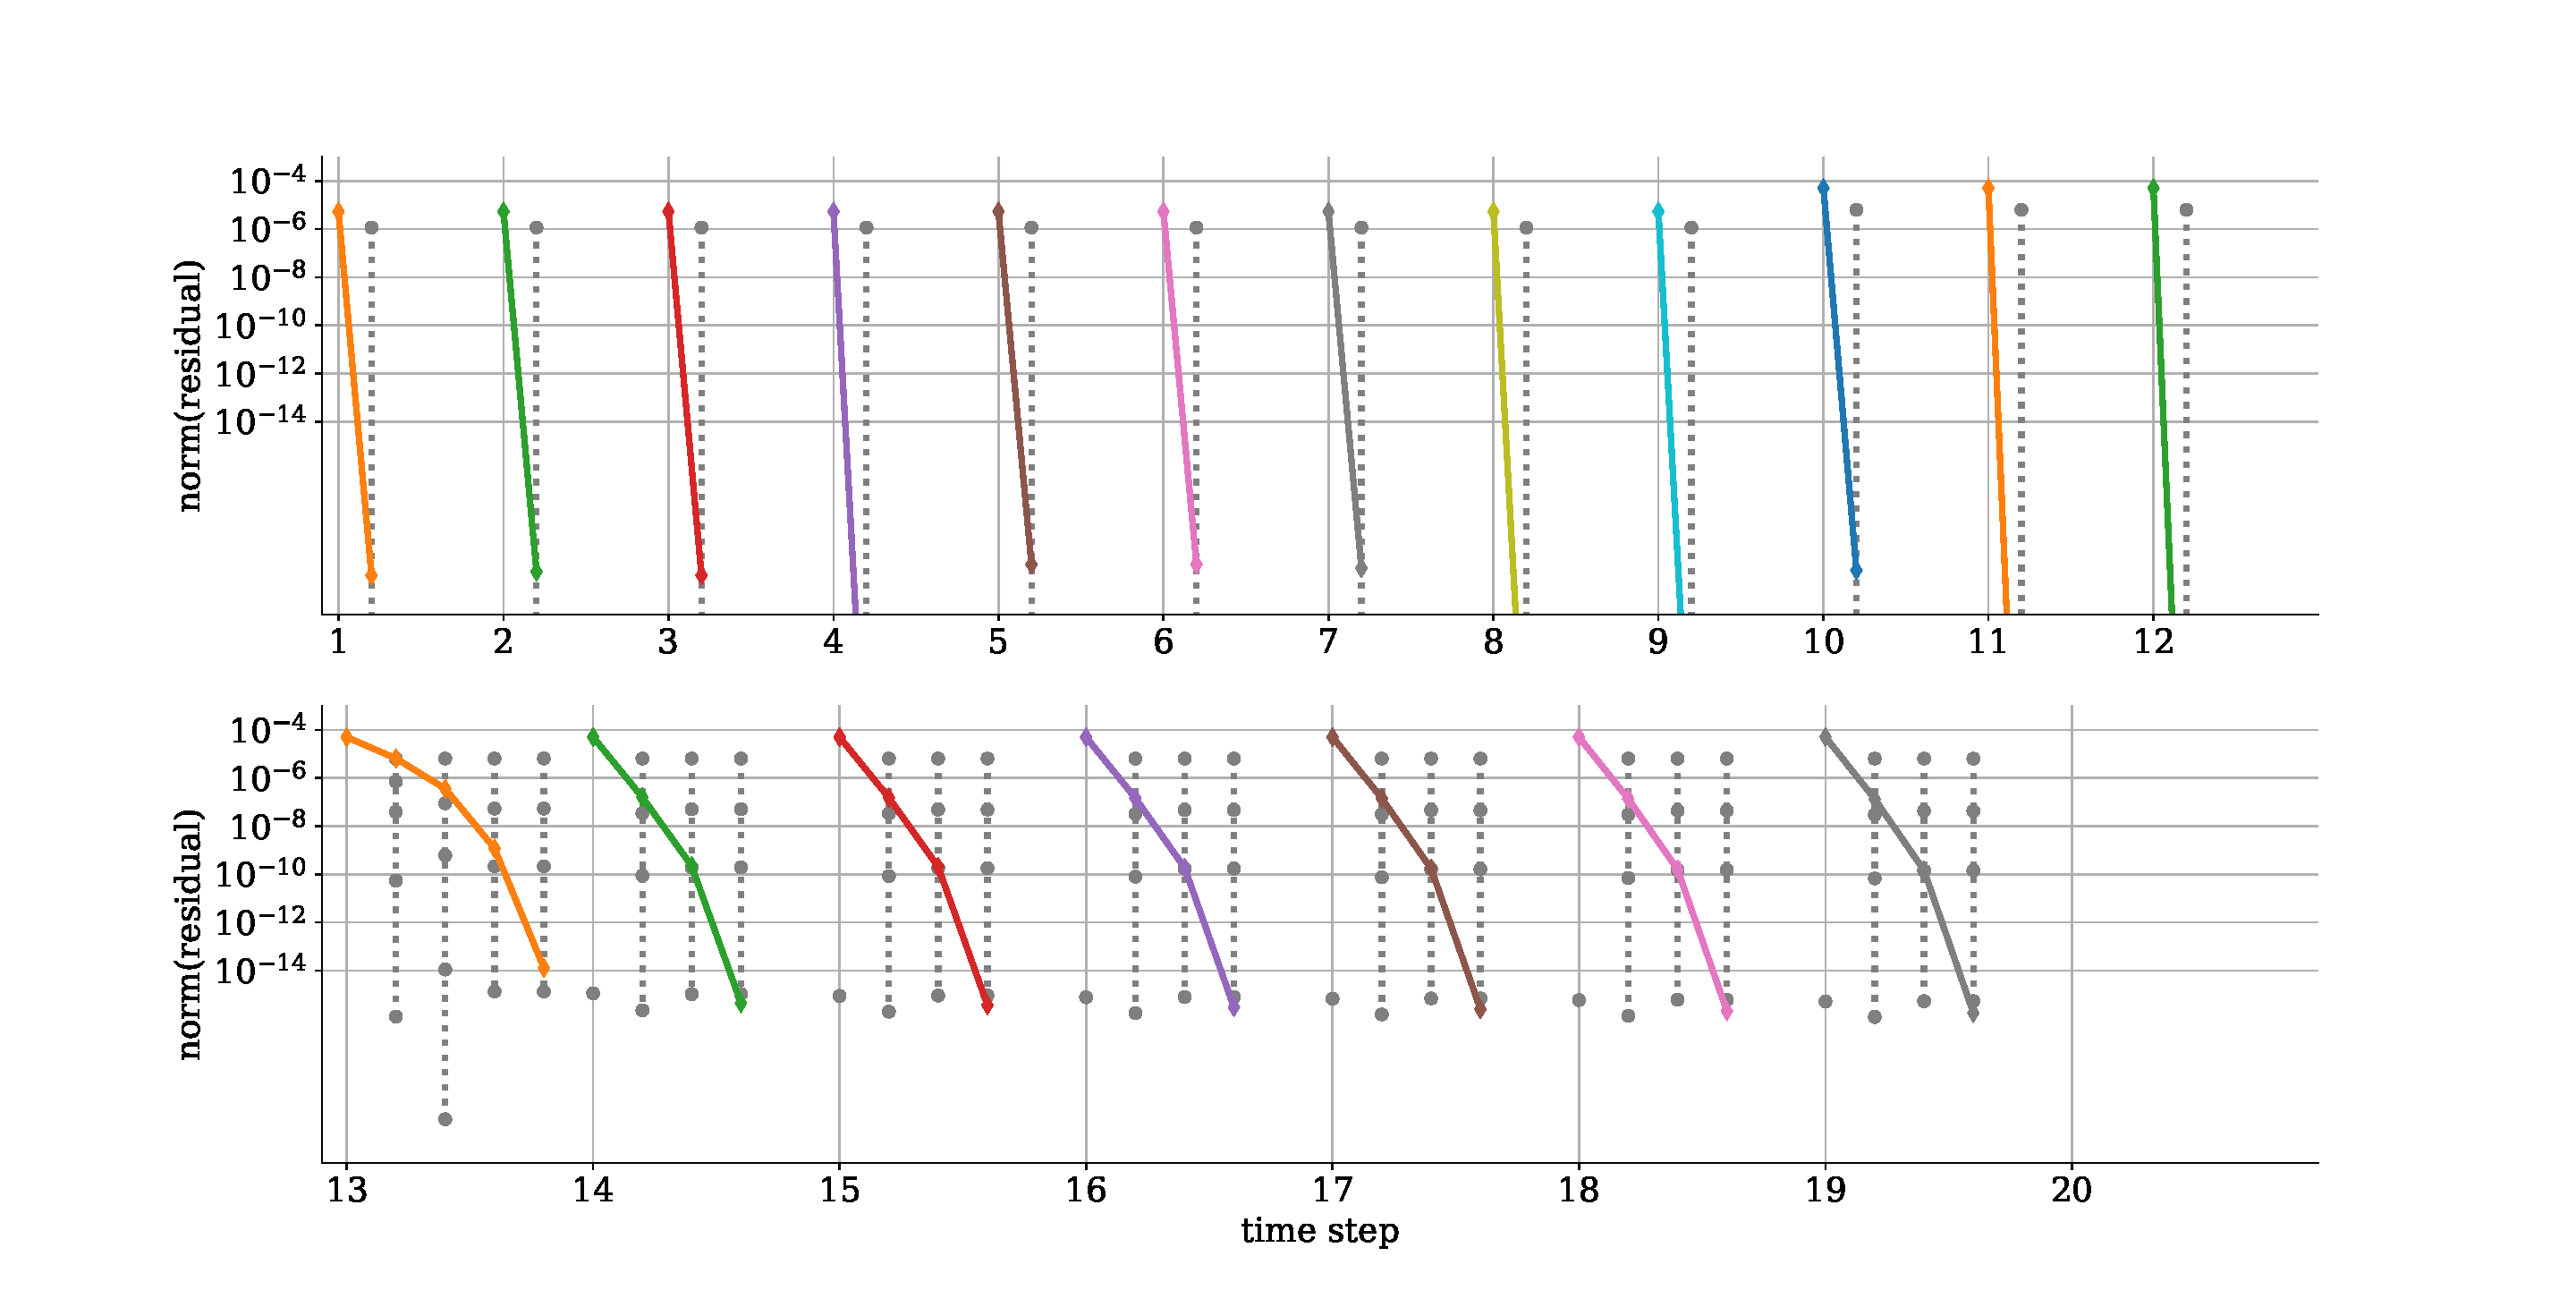
\includegraphics[width=1.04\textwidth]{img/SemiExplicitModifiedCamClay_OpenGeoSys2023/convergence_plot.pdf}
  \caption{Convergence plot: depicted is the norm of the residuals from the global iteration (colored) and the local iteration (grey) using the modified Cam clay \textsl{MFront} implementation \ref{subsec:ImplementationConstE} and \textsl{mtest}. Within the first $12$ steps the behavior is purely elastic (\textsl{top}), followed by contractant plastic flow (\textsl{bottom}).}\label{fig:convergencePlot}
\end{figure}

%with slight hardening (compaction)

As can be seen in \autoref{fig:convergencePlot}, convergence is achieved in one step in the elastic stage (\textsl{top}). In the plastic stage (\textsl{bottom}), the typical acceleration of convergence when approaching the solution is observed (asymptotic quadratic convergence). However, the convergence depends on the plastic flow behavior dictated by the parameters $M$, $\lambda\minus\kappa$ and $p_{\c0}$ and can reduce to super-linear (order $\in [1,2]$). 

%\pagebreak
\subsection{Orthotropic modified Cam clay model implementation}

Implementation \ref{subsec:ImplementationConstE} of the modified Cam clay model can be extended to orthotropic elastic behavior using the so-called standard bricks within \textsl{MFront}. Thus just one line of code need to be added:

\begin{lstlisting}[language={C++}]
@Brick StandardElasticity;
@OrthotropicBehaviour<Pipe>;
\end{lstlisting}

As a consequence the nine independent constants of orthotropic elasticity are already declared.

\begin{lstlisting}[language={C++}]
// material parameters
// Note: YoungModulus and PoissonRatio defined as parameters
// Note: Glossary names are already given; entry names are newly defined
@MaterialProperty real M;
@PhysicalBounds M in [0:*[;
M.setEntryName("CriticalStateLineSlope");
...
\end{lstlisting}

Since for Implementation \ref{subsec:ImplementationOriginal} the standard elasticity brick could not be used, more effort is required for the extension to orthotropic elasticity.

In any case, from the physical point of view it might be more realistic to consider the anisotropy both for the elastic and plastic behavior.

\subsection{Analytical expressions for porosity and pre-consolidation pressure evolution}
\label{subsec:AppSolutionPorosity}

Given is the evolution equation for the porosity:
\begin{equation}
  \dot{\phi} - \phi\divergence(\dot{\vec u}) = \trace(\dot{\tensor\varepsilon}) \quad\with\quad \varepsilon^\text{V} = \trace({\tensor\varepsilon}) \ .
\end{equation}
Exploiting $\divergence(\dot{\vec u})\equiv \trace(\dot{\tensor\varepsilon})$ and separating the variables yields the form
\begin{equation}
  \frac{\d\phi}{1-\phi} = \d\varepsilon^\text{V} \ .
\end{equation}
Integration over some time increment $\varDelta t$ with $\phi(t)={}^{k\!}\phi$ and $\phi(t+\varDelta t)={}^{k+1\!}\phi$ as well as $\Delta\varepsilon^\text{V}={}^{k+1\!}\varepsilon^\text{V}-{}^{k\!}\varepsilon^\text{V}$ as the volumetric strain increment, i.\,e.
\begin{equation}
  \int\limits_{{}^{k\!}\phi}^{{}^{k+1\!}\phi} \frac{\d\phi}{1-\phi} = \int\limits_{{}^{k\!}\varepsilon^\text{V}}^{{}^{k+1\!}\varepsilon^\text{V}} \d\varepsilon^\text{V} \ .
\end{equation}
then results in the incremental solution
\begin{equation}\label{eq:evolutionPhi}
  1 -\, {}^{k+1}\!\phi = (1-{}^{k}\!\phi) \exp(\minus\Delta\varepsilon^\text{V}) \ .
\end{equation}
Integration over the whole process time span with the initial values $\phi(t=0)={}^{0\!}\phi$ and $\varepsilon^\text{V}(t=0)=0$ results in
\begin{equation}\label{eq:totalEvolutionPhi}
  1-\phi = (1-{}^{0}\!\phi) \exp(\minus\varepsilon^\text{V}) \ .
\end{equation}
Combining \eqref{eq:totalEvolutionPhi} with \eqref{eq:evolutionPc} finally yields the evolution of the pre-consolidation pressure:
\begin{equation}
  \dot{p}_\c 
  = -\frac{\dot{\varepsilon}_\p^\text{V} p_\c}{(\lambda - \kappa)(1-{}^{0}\!\phi) \exp(\minus\varepsilon^\text{V})}
  \equiv \frac{v_0}{(\lambda - \kappa)} \exp(\varepsilon^\text{V})\, \dot{\varepsilon}_\p^\text{V} p_\c  \ .
\end{equation}
However, this equation is difficult to solve analytically. Therefore, and for the reasons explained in \autoref{subsec:PorosityEvolution}, the volume ratio is assumed almost constant as in Eq. \eqref{eq:linearEvolution}. Including the minimum value according to Eq. \eqref{eq:pcMin}, solving by separation of variables and integrating incrementally it is obtained
\begin{equation}\label{eq:pcIncrementalIntegration}
    {}^{k+1}p_\c = \left({}^k p_\c - p^\text{min}_\c\right) \exp\left(\minus\frac{v_0}{\lambda-\kappa}\left({}^{k+1}\varepsilon_\p^\text{V}-{}^k\varepsilon_\p^\text{V}\right)\right) + p^\text{min}_\c \ .
\end{equation}
This \emph{analytical} relation offers the possibility to eliminate the integration variable $p_\c$ completely and thus also the residual function $f_{p_\c}$. Of course, this has to be considered in the corresponding partial derivatives {(\ref{eqset:partialDerivatives}d--f)}. In a similar way, the \emph{analytical} Solution \eqref{eq:pIncrementalIntegration} for the pressure evolution can be used.
Such an implementation requires the consequent split of deviatoric and hydrostatic parts of the stress tensor, which also has to be considered in the partial derivatives. A (first) version of such an implementation called \texttt{ModCamClay\_semiExpl\_absP.mfront} was added to \textsl{OpenGeoSys}.


\subsection{Analytical solution of the Cam clay model for proportional loading}
\label{subsec:AppSolutionPeric}

A straight stress path from $(p,q)=(0, p_{\c0})$ until the final state $(p,q)=(387387, 330129)\ $Pa is considered:
\begin{equation}
    q = k\,(p-p_{\c0}) \ .
\end{equation}
The analytical solution \cite{Peric2006} for the corresponding equivalent strain $\varepsilon_{\text{q}}^2= {\tfrac{2}{3}\ \tensor\varepsilon^\D\ppkt\tensor\varepsilon^\D}$ reads
\begin{equation}
    \varepsilon_{\text{q}} = \varepsilon^\e_{\text{q}} + \varepsilon^\p_{\text{q}}
\end{equation}
and to be precise, using the abbreviations $C = (\lambda\minus\kappa)$ and $\alpha = 3(1-2\nu) / (2(1+\nu))$ it is
\begin{align}
    v_0\,\varepsilon^\e_{\text{q}} &= \ln\left[\left(1-\frac{q}{kp}\right)^{\frac{2Ck}{k^2-M^2}-\frac{\kappa k}{3\alpha}}\right]\ ,\\
    v_0\,\varepsilon^\p_{\text{q}} &= \ln\left[\left(1-\frac{q}{Mp}\right)^{\frac{Ck}{M(M-k)}} 
                                          \cdot\left(1+\frac{q}{Mp}\right)^{\frac{Ck}{M(M+k)}}\right]
                                          - 2 \frac{C}{M}\arctan\left(\frac{q}{Mp}\right)\ .
\end{align}

\subsection{Analytical considerations on pressure-dependent hypoelasticity}
\label{subsec:AppHypoelasticity}

Hypoelastic behavior with a pressure-dependent bulk modulus is considered. As pointed out before, there are two choices of which elastic parameter to keep constant (for isotropy):
\begin{enumerate}
    \item Assuming Poisson's ratio $\nu$ to be constant results in $G(p)$ (pressure dependent shear behavior).
    \item Assuming the shear modulus $G$ constant results in a pressure dependent $\nu$.
\end{enumerate}
For the first choice, the pressure-dependent elastic parameters read
\begin{equation}
  K(v,p) = \frac{v}{\kappa}p \quad,\quad G(v,p)=\frac{3(1-2\nu)}{2(1+\nu)}\,K(v,p) = \alpha(\nu) \,K(v,p) \ .
\end{equation}
Assuming the volume ratio almost constant (cf. \autoref{subsec:PorosityEvolution}) the dependency $v(\varepsilon^\text{V})$ can be ignored such that there is only $K(p), G(p)$. This facilitates the following derivation without changing the results significantly.
Then, the elastic stiffness tensor is not equal to the elasticity tensor anymore but has the form
\begin{align}
  \frac{\partial \tensor\sigma}{\partial \tensor\varepsilon_\e} &= 2G \tensorf J + 2\tensor\varepsilon_\e^\D \dyad  \frac{\partial G}{\partial p} \frac{\partial p}{\partial \varepsilon_\e^\text{V}} \frac{\varepsilon_\e^\text{V}}{\partial\tensor\varepsilon_\e} - \tensor I \dyad\frac{\partial p}{\partial \varepsilon_\e^\text{V}} \frac{\varepsilon_\e^\text{V}}{\partial\tensor\varepsilon_\e} \\
  &= 
  2G \tensorf J - 2\,\frac{v_0}{\kappa}\,\alpha(\nu) K\, \tensor\varepsilon_\e^\D \dyad \tensor I  - K \tensor I \dyad \tensor I \notag \\
  &= 
  2G \left\{\tensorf J - \frac{v_0}{\kappa}\, \tensor\varepsilon_\e^\D \dyad \tensor I \right\}  - K \tensor I \dyad \tensor I \ ,
\end{align}
where it was used that ${\partial p}/{\partial \varepsilon_\e^\text{V}}=-K$ and $G=\alpha(\nu)\,K$. Obviously, there is a one-sided pressure$\rightarrow$shear-coupling due to the pressure-dependent shear modulus. For this reason, major symmetry is lost. From the thermodynamic point of view this is a consequence of the \emph{hypo}elastic approach where no strain energy potential exists. Further note that an unsymmetric stiffness tensor implies energy sinks or sources.
\par
As an alternative, it is possible to keep the shear modulus $G$ constant. Then, ${\partial G}/{\partial p}=0$ and there is no (spurious) pressure$\rightarrow$shear-coupling. Moreover, the elastic stiffness tensor is symmetric and a convex strain energy potential now exists. However, Poisson's ratio implicitly becomes a function of the pressure because
\begin{equation}
  K(p) = \frac{v_0}{\kappa}p \quad,\quad \nu(p)=\frac{3K-2G}{2(3K+G)}
\end{equation}
and it must be ensured, that $\nu$ does not become negative for very small pressures (and thus low values of $K$). The hypoelastic relation \eqref{eq:evolutionP} for the pressure evolution can be solved analytically as shown in Section \ref{subsec:assumptions}. With this calculation of the hydrostatic pressure the stress tensor is composed to
\begin{equation}
  \tensor\sigma = 2G\,\tensor\varepsilon_\e^\D + (\minus p) \tensor I \ .    
\end{equation}
\par
It is important to note that the pressure dependence of the compression modulus is only reasonable for $p>0$ such that $K>0$. Moreover, a minimum value of $K$ must be guaranteed for numerical stability. Hence, it could be used
\begin{equation}
    p \overset{?}{<} p_0 \quad\leftrightarrow\quad \left(\varepsilon_\e^\text{V}-{}^0\varepsilon_\e^\text{V}\right)>0 \quad : \quad K = \frac{v}{\kappa}p_0 = \text{const.}
\end{equation}
Note that this version of the MCC model is not implemented in \textsl{OpenGeoSys} yet.


\printbibliography

\end{document}
